%% 
%% ACS project dissertation template. 
%% 
%% Currently designed for printing two-sided, but if you prefer to 
%% print single-sided just remove ",twoside,openright" from the 
%% \documentclass[] line below. 
%%
%%
%%   SMH, May 2010. 


\documentclass[a4paper,12pt,twoside,openright]{report}


%%
%% EDIT THE BELOW TO CUSTOMIZE
%%

\def\authorname{Zongzhe Yuan\xspace}
\def\authorcollege{Christ's College\xspace}
\def\authoremail{zy272@cl.cam.ac.uk}
\def\dissertationtitle{Extending CAS with Algebraic Reductions}
\def\wordcount{9,779}


\usepackage{epsfig,graphicx,parskip,setspace,tabularx,xspace} 
\usepackage{a4wide,parskip,times}
\usepackage{amsmath}
\usepackage{nicefrac}
\usepackage{ amssymb }
\usepackage{mleftright}
\usepackage{listings}

\usepackage[utf8]{inputenc}
\usepackage{amsfonts}
\usepackage{tikz}
\usetikzlibrary{arrows}
\usepackage{float}

\usepackage{fontspec}
\setmainfont{Latin Modern Roman}
\setmonofont{Latin Modern Mono}
\usepackage[title]{appendix}

\usepackage{minted}
\usemintedstyle{xcode}
\usepackage{libertine}
\usepackage{newunicodechar}
\newunicodechar{λ}{$\lambda$}
\newunicodechar{∀}{$\forall$}
\newunicodechar{→}{$\rightarrow$}

\newcommand{\e}[2]{
\begin{equation}
  \label{#1} 
  #2
\end{equation}
}


%% START OF DOCUMENT
\begin{document}


%% FRONTMATTER (TITLE PAGE, DECLARATION, ABSTRACT, ETC) 
\pagestyle{empty}
\singlespacing
% title page information
\begin{titlepage} 

\begin{center}
\noindent
\huge
\dissertationtitle \\
\vspace*{\stretch{1}}
\end{center}

\begin{center}
\noindent
\huge
\authorname \\
\Large
\authorcollege      \\[24pt]

\includegraphics{CUni3.eps}
\end{center}

\vspace{24pt} 

\begin{center}
\noindent
\large
{\it A dissertation submitted to the University of Cambridge \\ 
in partial fulfilment of the requirements for the degree of \\ 
Master of Philosophy in Advanced Computer Science} 
\vspace*{\stretch{1}}
\end{center}

\begin{center}
\noindent
University of Cambridge \\
Computer Laboratory     \\
William Gates Building  \\
15 JJ Thomson Avenue    \\
Cambridge CB3 0FD       \\
{\sc United Kingdom}    \\
\end{center}

\begin{center}
\noindent
Email: \authoremail \\
\end{center}

\begin{center}
\noindent
\today
\end{center}

\end{titlepage} 

\newpage
\vspace*{\fill}

\onehalfspacing
\newpage
{\Huge \bf Declaration}

\vspace{24pt} 

I \authorname of \authorcollege, being a candidate for the M.Phil in
Advanced Computer Science, hereby declare that this report and the
work described in it are my own work, unaided except as may be
specified below, and that the report does not contain material that
has already been used to any substantial extent for a comparable
purpose.

\vspace{24pt}
Total word count: \wordcount

\vspace{60pt}
\textbf{Signed}: 

\vspace{12pt}
\textbf{Date}:


\vfill

This dissertation is copyright \copyright 2018 \authorname. 
\\
All trademarks used in this dissertation are hereby acknowledged.



\newpage
\vspace*{\fill}

\singlespacing
\newpage
{\Huge \bf Abstract}
\vspace{24pt} 

This topic itself originated from the expansion of a routing problem that was not specifically reasoned in the L11 class. We classify this type of problem as the same problem, reduction. Although we discussed some of the properties of reduction in L11, we found that when we define the reduction we need, the construction of the reduction will conflict with the definition of reduction itself. Therefore, it shows that our definition of the reduction problem does not resolve our actual problem.

When we traced the source, we found reduction from a paper by Wongseelashote in 1979. Although Wongseelashote very skilfully proposed the concept of reduction when discussing path problems, it is regrettable that this paper does not provide detailed structural proof of reduction for its properties.

Therefore, our project is comprised of the following three parts. First of all, the classical reduction is expressed, and we are trying to reasoning the properties of reduction itself. Next, we will try to represent/define reduction in another way, not only to facilitate us to implement, but also to decrease the limitation of the reduction definition to practical problems. After that, we will define a kind of reduction according to requirements, and use this kind of reduction to construct numerous realistic examples. Finally, we will use these practical examples as a combination to solve the path problem mentioned in L11.

\newpage
\vspace*{\fill}


\pagenumbering{roman}
\setcounter{page}{0}
\pagestyle{plain}
\tableofcontents
\listoffigures
%\listoftables


\renewcommand{\lstlistlistingname}{List of Listings}
\addcontentsline{toc}{chapter}{\listoflistingscaption}%
\listof{listing}{\listoflistingscaption}%

\onehalfspacing

%% START OF MAIN TEXT 

\chapter{Introduction}
\pagenumbering{arabic} 
\setcounter{page}{1} 

%This is the introduction where you should introduce your work. In
%general the thing to aim for here is to describe a little bit of the
%context for your work --- why did you do it (motivation), what was the
%hoped-for outcome (aims) --- as well as trying to give a brief
%overview of what you actually did.
%
%It's often useful to bring forward some ``highlights'' into 
%this chapter (e.g.\ some particularly compelling results, or 
%a particularly interesting finding). 
%
%It's also traditional to give an outline of the rest of the
%document, although without care this can appear formulaic 
%and tedious. Your call. 

%Our dissertation problem originates from a concept that was mentioned in the L11 Algebraic Path Problem lecture, which has been introduced but not in detail \cite{griffin_2017}.  In the L11 lecture, the concept of reduction was proposed, with examples and was utilised to solve problems that we were unable to solve before. However, in addition to the definition of reduction provided in the lecture, the property of reduction has not been thoroughly discussed. Although we have found the definition of reduction and practical examples in other papers and theses before, unfortunately, none of them have discussed the property of reduction itself or provided a detailed, sound reasoning process.  This makes the detailed discussion of reduction a valuable research topic and thus becomes the topic of our project.
%
%In our research, we will not only conduct detailed reasoning on the properties of reduction, but we will also accomplish the following three goals:
%\begin{itemize}
%  \item The definition in L11 and the definition of reduction in the previous paper are all defined mathematically, which leads to the representation of reduction being difficult to implement. Therefore, we looked for an implementation-friendly representation equivalent to a traditional-reduction representation.
%  \item The functionality of classical reduction is limited, and it cannot represent some reductions (in particular, one of the reductions we used in the construction of our path problem). We will use a more generalised method to define reduction, generalise reduction, and evaluate its reasoning. 
%  \item Based on the application of reduction to real problems, we define predicate reduction on the basis of generalised reduction. Although predicate reduction is more concrete than generalised reduction (there are some reductions that cannot be represented by predicate reduction), it is a fairly generalised reduction and can be used to define many concrete instances of reduction. 
%\end{itemize}
%Finally, we will use predicate reduction combined with the properties of reduction, and some other mathematical structures, to define the path problem we encountered in the L11 lecture.

Combinators for algebraic systems (CAS) was introduced in the Mphil course L11 the Algebraic Path Problem \cite{griffin_2017}.
Those lectures briefly mentioned an algebraic construction called a 'reduction' that was first introduced by Wongseelashote in 1979\cite{WONGSEELASHOTE197955}.
This dissertation attempts to explore the reduction technique in depth.
In particular, we present the following contributions.
\begin{itemize}
  \item We develop a new representation of reductions called the full reduced representation, and show that this representation is isomorphic to the traditional representation of reductions introduced by Wongseelashote. Unlike the traditional representation, our representation  can be easily implemented in standard programming languages. See section \ref{def:full_reduced}.
  \item Motived by examples that arise by modelling internet routing protocols, we discover that we must generalise the theory of reduction.  See section \ref{def:generalised_reduction}.
  \item Again motived by internet routing protocols, we introduce a new family of generalized reduction. See section \ref{def:predicate_reduction}.
  \item Finally, all of our work was implemented by Coq theorem prover. This will be integrated into Dr Griffin's Coq based implementation of CAS. See section \ref{coq_implementation}.
\end{itemize}

Chapter \ref{background} introduces the algebraic background required. Our main contributions are described in Chapter \ref{main_contributions}, while conclusions are presented in the Chapter \ref{conclusion}. The appendix contains fragments of the Coq implementation, and the full implementation can be found in the associated file.

\chapter{Background} \label{background}

%A more extensive coverage of what's required to understand your 
%work. In general, you should assume the reader has a good undergraduate 
%degree in computer science, but is not necessarily an expert in 
%the particular area you've been working on. Hence this chapter 
%may need to summarize some ``text book'' material. 
%
%This is not something you'd normally require in an academic paper, 
%and it may not be appropriate for your particular circumstances. 
%Indeed, in some cases it's possible to cover all of the ``background'' 
%material either in the introduction or at appropriate places in 
%the rest of the dissertation. 

\section{Combinators for Algebraic System}
Combinators for Algebraic systems (CAS) evalued from the metarouting \cite{griffin_metarouting_2005}. It is a language for the design of algebraic systems, in which many algebraic properties are automatically infered, enabling people to combine different operators to obtain new structures. 
CAS includes the lexicographic product \cite{gurney_lexicographic_2007} which can be commonly found in metarouting protocol.

\section{Basic Definition}
 Let us begin with our problem set $S$, which is a collection of elements. Here in our project, we force our problem set $S$ to be non-trivial, which means there is at least one element inside the problem set.

\subsection{Equality}
In problem set $S$, the first thing we need to consider is the equality $=_S$. 
In the mathematical definition, we can think of equality as a particular binary relationship, which is a set of ordered pairs $=_S \in S \times S$. For equality, we have some properties that need to be discussed. 

Congruence: \e{def:eq:congruence}{\forall a,b,c,d \in S, a =_{S_1} b \wedge c =_{S_1} d \rightarrow a =_{S_2} c = b =_{S_2} d}
Reflexive: \e{def:eq:reflexive}{\forall a \in S, a =_S a}
Symmetric: \e{def:eq:symmetric}{\forall a,b \in S, a =_S b \rightarrow b =_S a}
Transitive: \e{def:eq:transitive}{\forall a,b,c \in S, a =_S b \wedge b=_S c \rightarrow a =_S c}

\subsection{Binary Operator}
The major focus of this project is binary operators on $S$. A binary operator $\oplus$ on $S$ is a function $\oplus : S \times S \rightarrow S$. The following properties of the binary operator will be discussed. 

Congruence: \e{def:bop:congruence}{\forall a,b,c,d \in S, a =_S b \wedge c =_S d \rightarrow a \oplus c =_S b \oplus d}
Associative: \e{def:bop:associative}{\forall a,b,c \in S, a \oplus (b \oplus c) =_S (a \oplus b) \oplus c}
Commutative: \e{def:bop:commutative}{\forall a,b \in S, a \oplus b =_S b \oplus a}
Not Commutative: \e{def:bop:not_commutative}{\exists a,b \in S, a \oplus b \neq_S b \oplus a}
Selective: \e{def:bop:selective}{\forall a,b \in S, a \oplus b =_S a \bigvee a \oplus b =_S b}
Left Distributive: Given another binary operator $\times : S \times S \rightarrow S$
\e{def:bop:left_distributive}{\forall a,b,c \in S, a \otimes (b \oplus c) =_S (a \otimes b) \oplus (a \otimes c)}
Not Left Distributive: Given another binary operator $\times : S \times S \rightarrow S$
\e{def:bop:not_left_distributive}{\exists a,b,c \in S, a \otimes (b \oplus c) \neq_S (a \otimes b) \oplus (a \otimes c)}
Right Distributive: Given another binary operator $\times : S \times S \rightarrow S$
\e{def:bop:right_distributive}{\forall a,b,c \in S, (a \oplus b) \otimes c =_S (a \otimes c) \oplus (b \otimes c)}
Not Right Distributive: Given another binary operator $\times : S \times S \rightarrow S$
\e{def:bop:not_right_distributive}{\exists a,b,c \in S, (a \oplus b) \otimes c \neq_S (a \otimes c) \oplus (b \otimes c)}

\section{Semiring and Path Problem}
The path problem has always fascinated mathematicians and computer scientists. 
At the very beginning, programmers and scientists designed algorithms to solve each path problem. 
The most famous path of these is the shortest distance problem and there are several well-known algorithms that can solve such problems: Dijkstra's algorithm, Bellman–Ford’s algorithm, A* search algorithm, and Floyd–Warshall’s algorithm \cite{cormen_introduction_2009}. 

%However, such an approach has its obvious shortcomings. At some point, designing a new algorithm can ‘steal’ the ideas of other algorithms, so people must redesign a completely new independent algorithm for each new problem (new metric).  This makes it difficult to use a generic (or framework) approach to solve this type of problem. Even if the path problem has minor changes, it is difficult for people to solve new problems by slightly modifying existing algorithms. 

People use different primitive metrics and various complicated algorithms to solve different path problems.
Hence, lots of predecessors have found algebraic approaches to resolve this kind of problem. 
Using the knowledge of abstract algebra, people find that the routing problems (path problems) can be represented using a mathematical structure called a ‘semiring’ $(S,\oplus,\otimes,\bar{0},\bar{1})$\cite{carre_algebra_1971,WONGSEELASHOTE197955,dynerowicz_forwarding_2013,mohri_semiring_2002,gurney_lexicographic_2007}. For example, the popular ‘shortest path problem’ can be represented as $(S, min,+,\infty,0)$\cite{mohri_semiring_2002} and the ‘maximal capacity path problem’ can be represented as $(S, max,min, 0, \infty)$. 

Before explaining our real problem, let us introduce a basic definition of a ‘semiring’. We will then discuss the reason that semiring can be applied to solve the path problem. 
\subsection{Semiring}
In abstract algebra, a semiring is a mathematical structure $(S,\oplus,\otimes,\bar0,\bar1)$ where $S$ is a set and $\oplus,\otimes$ are two binary operators $:S\times S \rightarrow S$.

$(S,\oplus)$ is a commutative semigroup (has associative property) and $(S,\otimes)$ is a semigroup:
\[
\forall a,b,c \in S, a \oplus (b\oplus c) = (a \oplus b) \oplus c,a \oplus b = b \oplus a
\]
\[
\forall a,b,c \in S, a \otimes (b\otimes c) = (a \otimes b) \otimes c
\]
$\oplus,\otimes$ are also left and right distributive on $S$: 
\[
\forall a,b,c \in S: a \otimes(b \oplus c) = (a \otimes b) \oplus (a \otimes c)
\]
\[
\forall a,b,c \in S:(a \oplus b) \otimes c  = (a \otimes c) \oplus (b \otimes c)
\] 
$\bar0$ is the identity of $\oplus$ and  $\bar1$ is the identity of $\otimes$: 
\[\forall a \in S, a \oplus \bar{0} = a = \bar{0} \oplus a\]
\[\forall a \in S, a \otimes \bar{1} = a = \bar{1} \otimes a\]
Finally, $\bar0$ is the  annihilator of $\otimes$: 
\[\forall a \in S, a \otimes \bar{0} = \bar{0} = \bar{0} \otimes a\]
Some definition will include that $\bar1$ is the annihilator of $\oplus$:
\[\forall a \in S, a \oplus \bar{1} = \bar{1} = \bar{1} \oplus a\]
Here we will include this property in our definition.
\subsection{Matrix Semiring and Stability}
For each semiring $(S,\oplus,\otimes,\bar0,\bar1)$ (that represent the metric of a path problem), we can define a matrix semiring $(M_n(S),\oplus,\otimes,\bar{J},\bar{I})$ to represent the configuration of a network. $M_n(S)$ is a $n\times n$ matrices over $S$,
\[(A \oplus B)(i,j) = A(i,j)\oplus B(i,j)\]
\[(A \otimes B)(i,j) = \bigoplus_{1\leq q \leq n}A(i,q)\otimes B(q,j)\]
\[\bar{J}(i,j) = \bar0\]
\[\bar{I}(i,j)=\left\{
\begin{array}{rcl}
\bar1       &      & {i = j}\\
\bar0     &      & {otherwise}
\end{array} \right.\]
So here, we can easily use this matrix to encode any specific path problem and use matrix multiplication to calculate a solution. 

For a directed graph $G = (V,E)$ and a weight function $w \in E \rightarrow S$, 
we can define the weight of a path $p = i_1,i_2, \dots i_k$ as $w(p) = w (i_1,i_2) \otimes w(i_2,i_3)\otimes \dots \otimes w(i_{k-1},i_k)$, while the empty path is given the weight of $\bar1$ and $\bar0$ stands for the infinite path (not path between two nodes).
Then we can define the adjacency matrix $A$ as: 
\[A(i,j)=\left\{
\begin{array}{rcl}
w(i,j)      &      & {(i,j)\in E}\\
\bar0     &      & {otherwise}
\end{array} \right.\]
And our problem will be represented as $A^*(i,j) = \bigoplus_{p \in \pi (i,j)}w(p)$.

However, our calculations depend on the properties of the semiring.

$a\in S$, we define the powers $a^k$ as, $a^0 = \bar{1}$ and $a^{k+1} = a \otimes a^k$.

$a\in S$, we define the closure $a^*$ as, $a^{(k)} = a^0 \oplus a^1 \dots  a^k$ and $a^* = a^0 \oplus a^1 \dots  a^k \oplus \dots$.

Here we say, if there exists a $q$ such that $a^{q} = a^{(q+1)}$, then $a$ is q-stable, which means $a^{q} = a^*$.

If we know that $S$ is 0-stable, then $M_n(S)$ is $n-1$-stable \cite{griffin_2017} (here we can ignore paths with loops, which is a reduction that will be introduced in a later section). 
This allows us to actually calculate, at most, $n-1$ steps, when calculating path problems.

Therefore, we can define the power and closure on the matrix semiring:

$A\in M_n(S)$,we define the powers $A^k$ as, $A^0 = \bar{I}$ and $A^{k+1} = A \otimes A^k$.

$A\in M_n(S)$,we define the closure $A^*$ as, $A^{(k)} = A^0 \oplus A^1 \dots  A^k$ and $A^* = A^0 \oplus A^1 \dots  A^k \oplus \dots$.


Hence, we have $\pi(i,j)$, which is the set of paths from $i$ to $j$, and $\pi^k(i,j)$ will be the set of paths from $i$ to $j$ with exactly $k$ arcs, and $\pi^{(k)}(i,j)$ will be the set of paths from $i$ to $j$ with at most $k$ arcs. Then we have:
\[A^k(i,j) = \bigoplus_{p \in \pi^k (i,j)}w(p)\]
\[A^{(k)}(i,j) = \bigoplus_{p \in \pi^{(k)} (i,j)}w(p)\]
\[A^*(i,j) = \bigoplus_{p \in \pi^* (i,j)}w(p)\]
It is worth mentioning that $A^*(i,j)$ may not be well-defined, but if $M_n(S)$ is $k$ stable, then for $A\in M_n(S)$, \[A^*(i,j) = A^{(k)}(i,j)\]

\subsection{Distributivity and Lexicographic Product}
The properties of distributivity (left and right) play an important role in the computation of the routing problem.
We have defined $M_n(S)$ the matrix and its related semiring on the given semiring $(S,\oplus,\otimes,\bar0,\bar1)$.
However, we still need to check the properties of $M_n(S)$, to make sure that it is exactly a semiring.
Considering the distributivity properties, $M_n(S)$ is left/right distributive if $S$ has distributivity properties.

Sometimes when we are defining complex routing problems, such as the widest-shortest path problem, constructed by a shortest path problem semiring and a widest path problem semiring using the lexicographic product, it is not guaranteed that the new data structure will still have the properties of distributivity. 

Suppose $(S,\oplus_S)$ is a commutative and selective semigroup and $(T,\oplus_t)$ is a semigroup, then the lexicographic product of two semigroups is $(S,\oplus_S) \bar{\times} (T,\oplus_T) = (S\times T, \oplus_{\bar{\times}})$ where
\[(s_1,t_1) \oplus_{\bar{\times}} (s_2,t_2)=\left\{
\begin{array}{rcl}
(s_1\oplus_S s_2,t_1\oplus_T t_2)      &      & { s_1 = s_1 \oplus_S s_2 = s_2}\\
(s_1\oplus_S s_2,t_1)       &      & {s_1 = s_1 \oplus_S s_2 \neq s_2}\\
(s_1\oplus_S s_2,t_2)       &      & {s_1 \neq s_1 \oplus_S s_2 = s_2}
\end{array} \right.\]

As mentioned above, we used the lexicographic product when constructing our final path problem and utilised the elementary path reduction. We also added a distinct annihilator to avoid excessive useless calculations. 

%These constructs make it difficult to speculate about the properties of our semiring (or new mathematical structure); this is why our project is devoted to research regarding the relationship between reduction and semiring properties.

\subsection{Global optimality vs. left/right local optimality}
On the other hand, we are required to discuss how to ensure our approach embraces the algebras that violate distributivity.

The global optimality: $A^*(i,j) = \bigoplus_{p \in \pi (i,j)}w(p)$,

The left local optimality: distributed Bellman-Ford algorithm: $L = (A\otimes L) \oplus \bar{I}$ which is $L(i,j) = \bigoplus_{q \in V} A(i,q)\otimes L(q,j)$,

The right local optimality: Dijkstra's algorithm: $R = (R\otimes A) \oplus \bar{I}$, which is  $L(i,j) = \bigoplus_{q \in V} R(i,q)\otimes A(q,j)$,

Noting that with distributivity, $M_n(S)$ is a semiring and the three optimality problems are essentially the same; the local optimal solutions are global solutions: $A^* = L = R$.

However, without distributivity, those three solutions may all exist distinctively,  and that brings us to the part of our project – discussing the relationship between reductions and semirings on distributive property.

\section{Classical Reduction, Example and Reasoning}
\subsection{Origin of the Concept of Reduction}
To better understand reduction and further analyse it in detail, we trace the source to find out if there are any other previous definitions and studies relating to reduction. 
The earliest definition we could find about reduction came from Ahnont Wongseelashote in 1979\cite{WONGSEELASHOTE197955}. Wongseelashote also encountered the problem similar to ours when studying the path problem in the paper. Our definition of reduction in L11 follows the step of Wongseelashoth in the paper.

Next, we found that Alexander James Telford Gurney also mentioned the concept of reduction in his Ph.D thesis\cite{gurney_construction_2010}. Gurney's discussion of reduction is founded on the definition by Wongseelashote and did not focus on reduction for detailed structure proof.

\subsection{Unary Operator}
The unary operator on $S$ will be used to express our reduction. A unary operator $r$ on $S$ is a function on $S$, $r : S \rightarrow S$. 
For unary operators, we are mainly interested in the following properties; these properties are also discussed later when reasoning the properties of reduction.

Congruence: \e{def:uop:congruence}{\forall a,b \in S, a =_S b \rightarrow r(a) =_S r(b)}
Idempotent: \e{def:uop:idempotent}{\forall a \in S, r(a) =_S r(r(a))}
Preserve Identity: Given a binary operator $\oplus : S \times S \rightarrow S$
\e{def:uop:preserve_id}{\exists i \in S, \forall a \in S, a \oplus i =_S a =_S i \oplus a \rightarrow r(i) =_S i}
Preserve Annihilator: Given a binary operator $\oplus : S \times S \rightarrow S$
\e{def:uop:preserve_ann}{\exists a \in S, \forall x \in S, x \oplus a =_S a =_S a \oplus x \rightarrow r(a) =_S a}
Left Invariant: Given a binary operator $\oplus : S \times S \rightarrow S$
\e{def:uop:left_invariant}{\forall a,b \in S, r(a) \oplus b =_S a \oplus b}
Right Invariant: Given a binary operator $\oplus : S \times S \rightarrow S$
\e{def:uop:right_invariant}{\forall a,b \in S, a \oplus r(b) =_S a \oplus b}

\subsection{Classical Reduction Definition}
Therefore, here we refer to the definition of reduction in L11 (also the definition of Wongseelashote in the paper) as the classical reduction, and we refer to the way it was represented by Wongseelashote as the traditional representation of reduction.
\begin{figure}[H]
\centering
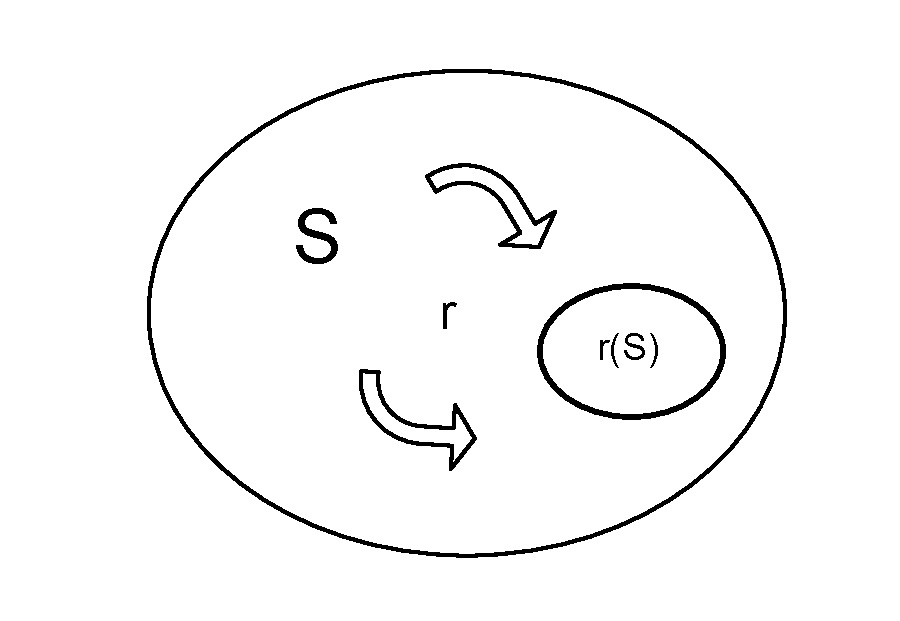
\includegraphics[width=0.8\textwidth]{reduction.pdf}
\label{reduction}
\caption{Illustration of Reduction}
\end{figure}
For a problem set $S$, the reduced problem set under reduction $r: S \rightarrow S$ is represented as 
\e{r:def:traditional}{r(S) \equiv \{s \in S | r(s) =_S s\}}
Then for the a semigroup $(S,=_S,\oplus)$, the reduced semigroup will be represented as \e{r:def:semirgoup}{{r(S) \equiv (\{s \in S | r(s) =_S s\}},=_S,\oplus_r)} and for two elements $a$ and $b$  in $r(S)$, we have 
\e{r:def:binary_operator}{a \oplus_r b \equiv r(a \oplus b)}
It is worth mentioning that although we use reduction to reduce the problem set from $S$ to $\{r(S) \equiv \{s \in S | r(s) =_S s\}$, our equality $=_S$ is still the original equality $=_S$. 
This can be seen from the figure (\ref{reduction}). Although we only focus on a subset of the original problem set $S$, the equality established in the problem set is still established in this subset. 
Here are the properties that a reduction $r$ needs to have \cite{WONGSEELASHOTE197955} :

Congruence: \e{r:def:congruence}{\forall a,b \in S, a =_S b \rightarrow r(a) =_S r(b)}
Idempotent: \e{r:def:idempotent}{r(a) = r(r(a))} 
Left Invariant: \e{r:def:left_invariant}{r(a\oplus b) = r(r(a)\oplus b) = r(a\oplus r(b))}
Right Invariant: \e{r:def:right_invariant}{r(a\otimes b) = r(r(a)\otimes b) = r(a\otimes r(b))}

\subsection{Example from the L11 Lecture}
For a given graph $G = (V,E)$, A cut set $C \in E$ for nodes $i$ and $j$ is a set of edges such there is no path from $i$ to $j$ in the graph $(V, E - C)$. $C$ is minimal if no proper subset of $C$ is a cut set. Martelli’s semiring \cite{martelli_gaussian_1976} is such that $A^{(*)}(i, j)$ is the set of all minimal cut sets for $i$ and $j$. 
So, Martelli’s semiring is represented as \[(S,\oplus,\otimes,\bar0,\bar1)\] where 
\[min_\leq \equiv \{ x \in X | \forall y \in X, y \not\leq x \}\]
\[S \equiv min_\leq(2^{2^E})\] 
\[X \hat{\cup} Y \equiv \{U \cup V | U \in X, V \in Y\}\]
\[X\oplus Y \equiv min_\leq(X \hat{\cup} Y)\] 
\[X\otimes Y \equiv min_\leq(X \cup Y)\] 
\[\bar0 \equiv \{\{\}\}\] 
\[\bar1 \equiv \{\}\]
The semiring uses two semirgoup reductions. $\oplus$ is the reduction $min_\leq$ over $\hat{\cup}$ and $\otimes$ is the reduction $min_\leq$ over $\cup$.
Here we can easily prove that $min_\leq$ satisfies our previous definition of reduction. So $min_\leq$ is a classical reduction.
\subsection{Reasoning on Classical Reduction}
Next, we need to make a detailed reasoning on the properties of the reduction.
Because we are talking about classical reduction, we assume that our reduction $r$ has properties of congruence (\ref{r:def:congruence}), idempotent (\ref{r:def:idempotent}), left invariant (\ref{r:def:left_invariant}) and right invariant (\ref{r:def:right_invariant}).

First, we discuss the properties of equality to the reduced problem set. We assume the equality $=_S$ has the properties of reflexive (\ref{def:eq:reflexive}), symmetric (\ref{def:eq:symmetric}), transitive (\ref{def:eq:transitive}), and congruence (\ref{def:eq:congruence}) on the original problem set $S$.
Then, because we have mentioned ‘although we use reduction to reduce the problem set from $S$ to $\{r(S) \equiv \{s \in S | r(s) =_S s\} $, we equality $=_S$ is still the original equality $=_S$’, the equality $=_S$ still has the property of reflexive, symmetric, transitive, and congruence on the reduced problem set $\{r(S) \equiv \{s \in S | r(s) =_S s\}$.

%Next, we need to discuss the properties of the binary operator under the reduced problem set. 
%Recalling our definition, for a binary operator $\oplus : S \times S \rightarrow S$, the reduced binary operator under reduction $r$ is defined as \[\forall a, b \in r(S) \equiv \{s \in S | r(s) =_S s\}, a \oplus_r b \equiv r(a \oplus b)\]
So, we first assume that the original binary operator $\oplus$ has certain properties on $S$, and then reasoning that these properties remain after reduction ($\oplus_r$ still has the same property under $\{r(S) \equiv \{s \in S | r(s) =_S s\}$).

Commutative: we initially assume that $\oplus$ is commutative under $S$, which is $\forall a,b \in S, a \oplus b =_S b \oplus a$. Then we want to prove that $\forall a,b \in \{s \in S | r(s) =_S s\}, a \oplus_r b =_S b \oplus_r a$.
\e{r:proof:commutative}{
\begin{array}{rcll} 
a \oplus_r b & =_S & r(a \oplus b) &\mbox{by the definition of $\oplus_r$} \\
			 & =_S & r(b \oplus a) &\mbox{by commutative of $\oplus$ and congruence of $r$}\\
             & =_S & b \oplus_r a &\mbox{by the definition of $\oplus_r$} \\
\end{array}}
So, we can conclude that commutative of $\oplus$ plus congruence of $r$ implies commutative of $\oplus_r$.

Congruence: we initially assume that $\oplus$ is congruence under $S$, which is $\forall a,b,c,d \in S, a =_S b \wedge c =_S d \rightarrow a \oplus c =_S b \oplus d$. Then we want to prove that $\forall a,b,c,d \in \{s \in S | r(s) =_S s\}, a =_S b \wedge c =_S d \rightarrow a \oplus_r c =_S b \oplus_r d$.
\e{r:proof:congruence}{
\begin{array}{rcll} 
a \oplus_r c & =_S & r(a \oplus c) &\mbox{by the definition of $\oplus_r$} \\
			 & =_S & r(b \oplus c) &\mbox{by congruence of $\oplus$ and congruence of $r$}\\
			 & =_S & r(b \oplus d) &\mbox{by congruence of $\oplus$ and congruence of $r$}\\
             & =_S & b \oplus_r d &\mbox{by the definition of $\oplus_r$} \\
\end{array}}
So, we can conclude that congruence of $\oplus$ plus congruence of $r$ implies congruence of $\oplus_r$.

Selective: we initially assume that $\oplus$ is selective under $S$, which is $\forall a,b \in S, a \oplus b =_S a \bigvee a \oplus b =_S b$. Then we want to prove that $\forall a,b \in \{s \in S | r(s) =_S s\}, a \oplus_r b =_S a \bigvee a \oplus_r b =_S b$. By using the selective property, we can split the cases of $a\oplus b$.

case 1: $a \oplus b =_S a$
\[
\begin{array}{rcll} 
a \oplus_r b & =_S & r(a \oplus b) &\mbox{by the definition of $\oplus_r$} \\
			 & =_S & r(a) &\mbox{congruence of $r$}\\
			 & =_S & a &\mbox{because $r(a) = a$}\\
\end{array}
\]
case 2: $a \oplus b =_S b$
\[
\begin{array}{rcll} 
a \oplus_r b & =_S & r(a \oplus b) &\mbox{by the definition of $\oplus_r$} \\
			 & =_S & r(b) &\mbox{congruence of $r$}\\
			 & =_S & b &\mbox{because $r(b) = b$}\\
\end{array}
\]
So, we can conclude that selective of $\oplus$ plus congruence of $r$ implies selective of $\oplus_r$.

Associative: we initially assume that $\oplus$ is associative under $S$, which is $\forall a,b,c \in S, a \oplus (b \oplus c) =_S (a \oplus b) \oplus c$. Then we want to prove that $\forall a,b,c \in \{s \in S | r(s) =_S s\}, a \oplus_r (b \oplus_r c) =_S (a \oplus_r b) \oplus_r c$. 
\e{r:proof:associative}{
\begin{array}{rcll} 
a \oplus_r (b \oplus_r c) & =_S & r(a \oplus r(b \oplus c)) &\mbox{by the definition of $\oplus_r$} \\
			 & =_S & r(a \oplus (b \oplus c)) &\mbox{by right invariant property of $r$ on $\oplus$}\\
			 & =_S & r((a \oplus b) \oplus c) &\mbox{by associative of $\oplus$ and congruence of $r$}\\
			 & =_S & r(r(a \oplus b) \oplus c) &\mbox{by left invariant property of $r$ on $\oplus$}\\
             & =_S & (a \oplus_r b) \oplus_r c  &\mbox{by the definition of $\oplus_r$} \\
\end{array}}
So, we can conclude that associative of $\oplus$ plus congruence, left and right invariant of $r$ on $\oplus$ implies associative of $\oplus_r$. Here we find that associative is not the same as the other three properties under binary operators. The proof that a binary operator satisfies the associative, under reduction, uses the left/right invariant properties of reduction. 

Left Distributive: by adding another binary operator $\otimes : S \times S \rightarrow S$, the reduced binary operator $\otimes_r$ as $\forall a,b \in \{s \in S | r(s) =_S s\}, a \otimes_r b \equiv r(a \otimes b)$, we initially assume that $\oplus$ and $\otimes$ are left distributive under $S$, which is $\forall a,b,c \in S, a \otimes (b \oplus c) =_S (a \otimes b) \oplus (a \otimes c)$. Then we want to prove that $\forall a,b,c \in \{s \in S | r(s) =_S s\}, a \otimes_r (b \oplus_r c) =_S (a \otimes_r b) \oplus_r (a \otimes_r c)$. 
\e{r:proof:left_distributive}{
\begin{array}{rcll} 
a \otimes_r (b \oplus_r c) & =_S & r(a \otimes r(b \oplus c)) &\mbox{by the definition of $\oplus_r$ and $\otimes_r$} \\
			 & =_S & r(a \otimes (b \oplus c)) &\mbox{by right invariant property of $r$ on $\otimes$}\\
			 & =_S & r((a \otimes b) \oplus (a \otimes c)) &\mbox{by left distributive of $\oplus$ and $\otimes$}\\
			 & =_S & r(r(a \otimes b) \oplus r(a \otimes c)) &\mbox{by left and right invariant of $r$ on $\oplus$}\\			 
			 & =_S & r((a \otimes_r b) \oplus (a \otimes_r c)) &\mbox{by the definition of $\otimes_r$}\\
             & =_S & (a \otimes_r b) \oplus_r (a \otimes_r c)  &\mbox{by the definition of $\oplus_r$} \\
\end{array}}
So, we can conclude that left distributive of $\oplus$ and $\otimes$ plus congruence, left and right invariant of $r$ on $\oplus$, right invariant of $r$ on $\otimes$ implies left distributive of $\oplus_r$ and $\otimes_r$.

Similarly, we can conclude that right distributive of $\oplus$ and $\otimes$ plus congruence, left and right invariant of $r$ on $\oplus$, left invariant of $r$ on $\otimes$ implies right distributive of $\oplus_r$ and $\otimes_r$.

Thus, we conclude that a distributive of $\oplus$ and $\otimes$ plus congruence, left and right invariant of $r$ on $\oplus$ and $\otimes$ implies a distributive of $\oplus_r$ and $\otimes_r$.
It is also worth mentioning that the property of the distributive is one of the major features that will be discussed in the later section.

%\chapter{Related Work} 
%
%This chapter covers relevant (and typically, recent) research 
%which you build upon (or improve upon). There are two complementary 
%goals for this chapter: 
%\begin{enumerate} 
% \item to show that you know and understand the state of the art; and 
% \item to put your work in context
%\end{enumerate} 
%
%Ideally you can tackle both together by providing a critique of
%related work, and describing what is insufficient (and how you do
%better!)
%
%The related work chapter should usually come either near the front or
%near the back of the dissertation. The advantage of the former is that
%you get to build the argument for why your work is important before
%presenting your solution(s) in later chapters; the advantage of the
%latter is that don't have to forward reference to your solution too
%much. The correct choice will depend on what you're writing up, and
%your own personal preference.

\chapter{Main Contributions} \label{main_contributions}

%This chapter may be called something else\ldots but in general 
%the idea is that you have one (or a few) ``meat'' chapters which
%describe the work you did in technical detail. 

\section{New Reduction Representation}\label{def:full_reduced}
It is obvious that the definition of classical reduction traditional representation is not implementation friendly.
This is because the traditional reduction representation depicts the actual problem set as $r(S) = \{s\in S|r(s)=_S s\}$ which is a type with record . It is difficult to accurately represent records in most situations. 

Imagine we have two different reductions $r_1$ and $r_2$ for $S$, then the problem set after applying reduction $r_1$ and $r_2$ will be $r_2(r_1(S)) = \{y\in \{x \in S | r_1(x) =_S x\}|r_2(y)=_S y\}$. 

The nested  record of reduction in our problem domain creates problems with the reasoning and calculation steps. 
At the same time, since our real problem set has changed from the original $S$ to the current $r(S) = \{s\in S|r(s)=_S s\}$ (suppose we only have one reduction $r$), the domain of our binary operator has changed. If we originally have a binary operator $\oplus : S\times S \rightarrow S$, then the binary operator after reduction will become the binary operator \[\oplus_r : \{s\in S|r(s)=_S s\} \times \{s\in S|r(s)=_S s\} \rightarrow \{s\in S|r(s)= s\}\] If we apply two/more reductions simultaneously, the entangling of reductions with the problem set and operator makes it almost impossible for us to define the combinator that exists on reduction and solve the problem at all.

Our goal is to redefine the equality and binary operators without changing the problem set $S$. 
Then the reduced problem set based on $(S,=_S,\oplus)$ by reduction $r$ will become $(S,=^r_S,\oplus^r)$, which is still a problem set on $S$, but not $(\{x \in S | r(x) =_S x\}, =,\oplus_r)$. 
Then we will prove the isomorphism between these two representations.
\[
\begin{array}{rcll}
(S,=_S,\oplus) & \longrightarrow & (\{x \in S | r(x) =_S x\}, =,\oplus_r) & \mbox {traditional representation}\\
(S,=_S,\oplus) & \longrightarrow & (S,=^r_S,\oplus^r) & \mbox{full reduction representation}
\end{array}
\]

\subsection{Full Reduction Representation}
Let us look back at the figure (\ref{reduction}). In the figure, our reduction will reduce the problem set $S$ to a subset of $S$. In our traditional representation, because reduction has already brought the problem set from $S$ to $\{x \in S | r(x) =_S x\}$, which means when we are comparing two elements from the problem set, those two elements are already inside $\{x \in S | r(x) =_S x\}$, we can also directly use the original equality $=_S$.

However, if we want to keep our problem set unchanged as $S$, when we are doing an equality comparison, we must guarantee that the elements we compared are already inside the reduced problem set. Thus, we define the new equality as, for all $a$ and $b$ in $S$,
\e{gr:def:eq}{a =^r_S b \equiv r(a) =_S r(b)}
The same reason applies for our binary operator  $\oplus$, because the arguments we need have been reduced to $\{x \in S | r(x) =_S x \}$ for our previous defined $\oplus_r$, we only need to consider that the result of operation must also be in $\{x \in S | r(x) =_S x\}$, so we give the definition above (\ref{r:def:binary_operator}).
But now, if we want to keep our problem set unchanged as $S$, when we are doing binary operations, we not only need to consider that the result of the operation is in the reduced problem set, but also to ensure that the two arguments of the binary operator are in the reduced problem set. Therefore, we define our binary operator under reduction: For all elements $a$ and $b$ in $S$,
\e{gr:def:binary_operator}{a \oplus^r b \equiv r(r(a) \oplus r(b))}
We call this representation as full reduction because we applied the reduction to both arguments $a$ and $b$ since we can't assume that the already reduced, and to the result of the calculation.


\subsection{Isomorphism between Traditional and Full Reduction Representation}
Next, we need to prove that our new full reduction representation is isomorphic to the previous traditional representation.

\subsubsection{Isomorphic on Equality Properties}
First, we discuss the properties on equality between the traditional representation and the full reduction representation.

Congruence: we need to prove that $=_S$ is congruence on $\{x \in S | r(x) =_S x\}$ is isomorphic to $=^r_S$ is congruence on $S$, which means 
\[\forall a,b,c,d \in \{x \in S | r(x) =_S x \}, a =_S b \wedge c =_S d \rightarrow a =_S c = b =_S d \]
\[\longleftrightarrow \]
\[\forall a,b,c,d \in S, a =^r_S b \wedge c =^r_S d \rightarrow a =^r_S c = b =^r_S d
\]

Reflexive: we need to prove that $=_S$ is reflexive on $\{x \in S | r(x) =_S x \}$ is isomorphic to $=^r_S$ is reflexive on $S$, which means 
\[\forall a \in \{x \in S | r(x) =_S x \}, a =_S a \]
\[\longleftrightarrow \]
\[\forall a \in S, a =^r_S a
\]

Symmetric: we need to prove that $=_S$ is symmetric on $\{x \in S | r(x) =_S x\}$ is isomorphic to $=^r_S$ is symmetric on $S$, which means 
\[\forall a,b \in \{x \in S | r(x) =_S x \}, a =_S b \rightarrow b =_S a \]
\[\longleftrightarrow \]
\[\forall a,b \in S, a =^r_S b \rightarrow b =^r_S a
\]

Transitive: we need to prove that $=_S$ is transitive on $\{x \in S | r(x) =_S x \}$ is isomorphic to $=^r_S$ is transitive on $S$, which means 
\[\forall a,b,c \in \{x \in S | r(x) =_S x \}, a =_S b \wedge b =_S c \rightarrow a =_S c \]
\[\longleftrightarrow \]
\[\forall a,b,c \in S, a =^r_S b \wedge b =^r_S c \rightarrow a =^r_S c
\]

This proof is really trivial and only needs the property of idempotent of $r$, which is $\forall a \in S, r(a) = r(r(a))$. 

\subsubsection{Isomorphic on Binary Operator Properties}
Next, we are going to discuss the properties on binary operator $\oplus$ (and $\otimes$ when we are talking about distributive) between the traditional representation and the full reduction representation.

Commutative: we need to prove that $\oplus_r$ is commutative on $\{x \in S | r(x) =_S x\}$ is isomorphic to $\oplus^r$ is commutative on $S$, which means 
\[\forall a,b \in \{x \in S | r(x) =_S x \}, a \oplus_r b =_S b \oplus_r a \]
\[\longleftrightarrow \]
\[\forall a,b \in S, a \oplus^r b =^r_S b \oplus^r a
\]

Selective: we need to prove that $\oplus_r$ is selective on $\{x \in S | r(x) =_S x\}$ is isomorphic to $\oplus^r$ is selective on $S$, which means 
\[\forall a,b \in \{x \in S | r(x) =_S x\}, a \oplus_r b =_S a \bigvee a \oplus_r b =_S b \]
\[\longleftrightarrow \]
\[\forall a,b \in S, a \oplus^r b =^r_S a \bigvee a \oplus^r b =^r_S b
\]

Congruence: we need to prove that $\oplus_r$ is congruence on $\{x \in S | r(x) =_S x\}$ is isomorphic to $\oplus^r$ is congruence on $S$, which means 
\[\forall a,b,c,d \in \{x \in S | r(x) =_S x \}, a =_S b \wedge c =_S d \rightarrow a \oplus_r c =_S b \oplus_r d \]
\[\longleftrightarrow \]
\[\forall a,b,c,d \in S, a =^r_S b \wedge c =^r_S d \rightarrow a \oplus^r c =^r_S b \oplus^r d
\]

Associative: we need to prove that $\oplus_r$ is associative on $\{x \in S | r(x) =_S x\}$ is isomorphic to $\oplus^r$ is associative on $S$, which means 
\[\forall a,b,c \in \{x \in S | r(x) =_S x \}, a \oplus_r (b \oplus_r c) =_S (a \oplus_r b) \oplus_r c \]
\[\longleftrightarrow \]
\[\forall a,b,c \in S, a \oplus^r (b \oplus^r c) =^r_S (a \oplus^r b) \oplus^r c
\]

Left Distributive: we need to prove that $\oplus_r$ and $\otimes_r$ are left distributive on $\{x \in S | r(x) =_S x\}$ is isomorphic to $\oplus^r$ and $\oplus^r$ are left distributive on $S$, which means 
\[\forall a,b,c \in \{x \in S | r(x) =_S x \}, a \otimes_r (b \oplus_r c) =_S (a \otimes_r b) \oplus_r (a \otimes_r c) \]
\[\longleftrightarrow \]
\[\forall a,b,c \in S, a \otimes^r (b \oplus^r c) =^r_S (a \otimes^r b) \oplus^r (a \otimes^r c)
\]

Right Distributive: we need to prove that $\oplus_r$ and $\otimes_r$ are right distributive on $\{x \in S | r(x) =_S x\}$ is isomorphic to $\oplus^r$ and $\oplus^r$ are right distributive on $S$, which means 
\[\forall a,b,c \in \{x \in S | r(x) =_S x \}, (a \oplus_r b) \otimes_r c =_S (a \otimes_r c) \oplus_r (b \otimes_r c) \]
\[\longleftrightarrow \]
\[\forall a,b,c \in S, (a \oplus^r b) \otimes^r c =^r_S (a \otimes^r c) \oplus^r (b \otimes^r c)
\]

This proof will be shown in the Coq \cite{Coq} file and we only need the property of congruence and idempotent of $r$, which is $\forall a \in S, r(a) = r(r(a))$ and $\forall a,b \in S, a =_S b \rightarrow r(a) =_S r(b)$.

This proves that our full reduction representation of reduction is isomorphic to the traditional representation of reduction, which means all the properties we have proved in the classical reduction section using traditional representation could be used directly in our full reduction representation.


\section{Generalised Reduction}\label{def:generalised_reduction}
In this section, we consider the need to generalise the classical reduction.
\subsection{Motivating Example}
%For each path problem that is represented as a semiring, we can construct a corresponding matrix semiring that represents the concrete problem (for example, the edges and the distances for the shortest path problem). Then, using matrix multiplication and stability of the closure (the semiring), we can solve the real problem of each concrete path problem. However, the simple matrix approach can only solve ‘trivial’ path problems. Complicated problems, for example, the widest shortest path problem that was constructed from the shortest path problem semiring and the widest path problem (maximal capacity path problem) semiring using the lexicographic product, cannot be solved by this ‘traditional’ theory approach. Sometimes, even the method can find an optimal solution; there are no guarantees that all optimal solutions will be found using the classic method.

%Therefore, a non-classical algebraic path-finding method is used, so algebras that violate the distribution law can be accepted.  This non-classical theory can handle problems that the simple classical theory cannot handle, such as the problems that cannot be solved by Dijkstra or Bellman-Ford.
%This kind of method is dedicated, initially, to finding the local optimal solution. The local optimal solution is exactly the same as the global optimal solution by some verification or some additional restriction on the computation. For instance, the famous routing information protocol, which is based on distributed Bellman-Ford algorithms, is a non-traditional theory.
%Here, we provide two examples; if we follow the basis of distributed Bellman-Ford algorithm Protocol \cite{hedrick_routing_1988} that calculates the path from $i$ to destination $j$, using the knowledge from its immediate neighbourhood and applying its own path to the neighbour available in the process, we will obtain the result using matrix multiplication. 

Consider the figure in \ref{example:rip:1} taken from the RIP protocol \cite{hedrick_routing_1988}. 

\begin{figure}[H]
\centering
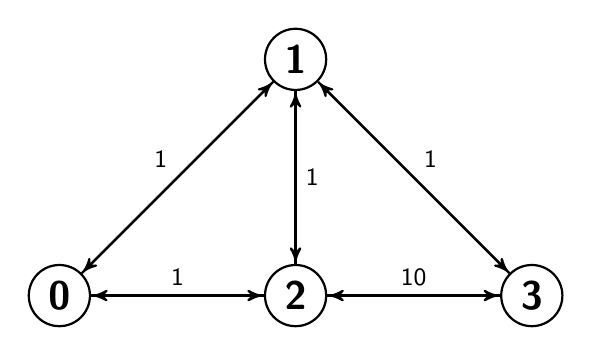
\begin{tikzpicture}[->,>=stealth',shorten >=1pt,auto,node distance=3cm,
                    thick,main node/.style={circle,draw,font=\sffamily\Large\bfseries}]

  \node[main node] (0) {0};
  \node[main node] (2) [right of=0] {2};
  \node[main node] (1) [above of=2] {1};
  \node[main node] (3) [right of=2] {3};

\path[every node/.style={font=\sffamily\small}]
    (0) edge node {1} (2)
        edge node {1} (1)
	(1) edge node {} (0)
        edge node {1} (2)
        edge node {1} (3)
    (2) edge node {} (0)
        edge node {} (1)
        edge node {10} (3)
    (3) edge node {} (2)
        edge node {} (1)
;
\end{tikzpicture}
\label{example:rip:1}
\caption{Example of RIP solution 1}
\end{figure}
This can be described with an adjacency matrix over $(\mathbb{N},min,+)$ semiring.
\[A_1 =
\begin{bmatrix}
    \infty & 1 & 1 & \infty \\
    1 & \infty & 1 & 1 \\
    1 & 1 & \infty & 10 \\
    \infty & 1 & 10 & \infty \\
\end{bmatrix}
\]
RIP is a distributive Bellman–Ford’s protocol. Abstractly, we can model this by iterating matrix multiplication. In several iterations, we will obtains solutions.
\[A^*_1 =
\begin{bmatrix}
    0 & 1 & 1 & 2 \\
    1 & 0 & 1 & 1 \\
    1 & 1 & 0 & 2 \\
    2 & 1 & 2 & 0 \\
\end{bmatrix}
\]
%\begin{figure}[H]
%\centering
%\begin{tikzpicture}[->,>=stealth',shorten >=1pt,auto,node distance=3cm,
%                    thick,main node/.style={circle,draw,font=\sffamily\Large\bfseries}]
%
%  \node[main node] (0) {0};
%  \node[main node] (2) [right of=0] {2};
%  \node[main node] (1) [above of=2] {1};
%  \node[main node] (3) [right of=2] {3};
%
%\path[every node/.style={font=\sffamily\small}]
%    (0) edge node {1} (2)
%        edge node {1} (1)
%	(1) edge node {} (0)
%        edge node {1} (2)
%    (2) edge node {} (0)
%        edge node {} (1)
%        edge node {10} (3)
%    (3) 
%        edge node {} (2)
%;
%\end{tikzpicture}
%\label{example:rip:2}
%\caption{Example of RIP solution 2}
%\end{figure}
%Then for example 2, we will get the following initial path problem adjacency matrix.
%\[
%\begin{bmatrix}
%    \infty & 1 & 1 & \infty \\
%    1 & \infty & 1 & \infty \\
%    1 & 1 & \infty & 10 \\
%    \infty & \infty & 10 & \infty \\
%\end{bmatrix}
%\]
%After using the RIP protocol for matrix calculations (multiplication), we obtained such an adjacency matrix as the result:
%\[
%\begin{bmatrix}
%    0 & 1 & 1 & 11 \\
%    1 & 0 & 1 & 11 \\
%    1 & 1 & 0 & 10 \\
%    11 & 11 & 10 & 0 \\
%\end{bmatrix}
%\]

\subsection{Previous Problem in L11}
%However, RIP will also have a series of problems. For example, when a node has no edges connected to all other nodes, the RIP matrix calculation (without pre-limiting the maximum number of calculation steps) will continue infinitely. Even if the maximum number of calculation steps is set in advance, RIP still has some deficiencies. 
%This leads to the problem that not all real-world problems can be solved directly using the simple matrix semiring. 
%For instance, we may meet the following situation where node 3 is not connected to all other nodes.

Supposed that RIP has converged on the solution $A^*_1$. Now imagine the links on node 3 fail.

\begin{figure}[H]
\centering
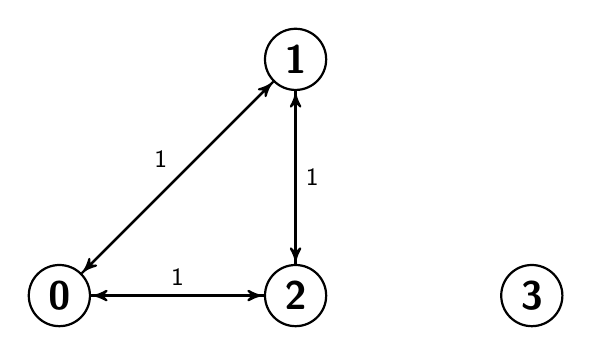
\begin{tikzpicture}[->,>=stealth',shorten >=1pt,auto,node distance=3cm,
                    thick,main node/.style={circle,draw,font=\sffamily\Large\bfseries}]

  \node[main node] (0) {0};
  \node[main node] (2) [right of=0] {2};
  \node[main node] (1) [above of=2] {1};
  \node[main node] (3) [right of=2] {3};

\path[every node/.style={font=\sffamily\small}]
    (0) edge node {1} (2)
        edge node {1} (1)
	(1) edge node {} (0)
        edge node {1} (2)
    (2) edge node {} (0)
        edge node {} (1)
;
\end{tikzpicture}
\label{example:rip:2}
\caption{Example of RIP solution 2}
\end{figure}
Since RIP is a distributive protocol, there is no way to restart from the 'true' adjacency matrix
\[A_2 = 
\begin{bmatrix}
    0 & 1 & 1 & \infty \\
    1 & 0 & 1 & \infty \\
    1 & 1 & 0 & \infty \\
    \infty & \infty & \infty & 0 \\
\end{bmatrix}
\]
Instead, it starts the iteration in the state of $A^*_1$.
After using the RIP protocol for n-step matrix calculations (multiplication), a matrix such as this was obtained:
\[
\begin{bmatrix}
    0 & 1 & 1 & n+1 \\
    1 & 0 & 1 & n+1 \\
    1 & 1 & 0 & n+1 \\
    \infty & \infty & \infty & 0 \\
\end{bmatrix}
\]
The result shows that if we do not limit the number of steps in the calculation, even though we may get the results of the path we need in the early steps (e.g. the path from $a$ to $b$), but a better solution for the entire matrix may be found after many steps (or the calculation will be infinite, which is shown in this example). 
\subsection{Adding Explicit Path to Shortest Pat}
Therefore, in the course of L11, instead of using RIP and a simple matrix semiring approach, we used another protocol called BGP \cite{rekhter_application_1991}. We started from the simple $(\mathbb{N},min,+)$ semiring that calculated the shortest distance and used the lexicographic product to construct a new semiring that contained the shortest-path metric and the set of its path.

Here we need to define some new operators/new rules for our semigroup.
Assume $(S,\bullet)$ is a semigroup. Let
\begin{equation}
  \label{eq:lift:def} 
  lift(S,\bullet) \equiv (fin(2^S),\hat\bullet)
\end{equation}   
where
$X \hat\bullet Y = \{x\bullet y |x\in X,y\in Y\}$.

Then we can use our $lift$ to construct a bi-semigroup.
Assume $(S,\bullet)$ is a semigroup. Let
\begin{equation}
  \label{eq:unionlift:def} 
  union\_lift(S,\bullet)\equiv (\mathcal{P}(S),\cup,\hat\bullet)
\end{equation}  
where
$X \hat\bullet Y = \{x\bullet y |x\in X,y\in Y\}$, and $X,Y \in \mathcal{P}(S)$, which is the set of finite subsets of $S$.

Note that the empty set $\{\}$ is the additive identity and the multiplicative annihilator.

Then for a given graph $G = (V,E)$, we define
\begin{equation}
  \label{eq:path:def} 
  path(E)\equiv union\_lift(E^*,.) 
\end{equation}  
where . is the concatenation function of the sequence.

Finally, we get our ‘shortest paths with paths’ semiring from a given graph $G = (V,E)$: 
\begin{equation}
  \label{eq:spwp:def} 
  spwp \equiv AddZero(\infty,(\mathbb{N},min,+) \overrightarrow{\times} path(E))
\end{equation} 

\subsection{Introduce Reduction into Our Problem}
We come to a problem when we are using $spwp$ for doing calculations; because there may be loops in our $path(E)$, we need a lot of extra computation to prove that the paths that have loops are not the shortest paths.
To eliminate these paths with loops, we introduced the reduction into our problem.

For a given path $p$, we say $p$ is elementary if there is no node inside $p$ that is repeated. Then we can define our elementary path using the reduction 
\e{r:def:elementary}{r(X) = \{p\in X | p \mbox{ is elementary }\}}and 
\e{r:def:elementary_path}{epaths(E) = red_r(paths(E))}

The reduction on the additive component does not follow the property of the reduction on the $min$ operation (it does not have left/right invariant property). Imagine we have path $A = \{a,b,c,d\}$ that is longer but does not have loop and $B = \{a,b,b\}$ that is shorter path but does have loop. Then $r(A\oplus B) = r(B) = \infty$ because $B$ is shorter but has a loop, but $r(A\oplus r(B)) = r(A \oplus \infty) = r(A) = A$ because $B$ has loops but $A$ does not. 
Note that this is new. The presentation in L11 did not go into any detailed there, and did not realized that a generalized of reduction will resolve the problem.
This is the problem we will resolve in the next section \ref{gr:def}.



Therefore, our path problem semiring becomes 
\e{r:def:path_problem}{AddZero(\infty,(\mathbb{N},min,+) \overrightarrow{\times} epath(E))}

However, we still encounter the problem that there exists elements in our problem set that have a path distance value but do not have edges in their path. This iteration can go forever, since all paths have loops in them, and the empty set is legitimate second component for our algebra.

\[
\begin{bmatrix}
    (0,\{\epsilon\}) & (1,\{(0,1)\})    & (1,\{(0,2)\})   & (n+1,\{\}) \\
    (1,\{(1,0)\})    & (0,\{\epsilon\}) & (1,\{(1,2)\})   & (n+1,\{\}) \\
    (1,\{(2,0)\})    & (1,\{(2,1)\})    & (0,\{\epsilon\})& (n+1,\{\}) \\
    \infty           & \infty           & \infty          & (0,\{\epsilon\}) \\
\end{bmatrix}
\]

So, we need to define the second reduction, which turns all elements that have $\{\}$ as the second component into $\infty$.
\e{r:def:reduction_annihilator}{
\begin{array}{rcl} 
r_2 (inr(\infty)) & = & inr(\infty) \\
r_2 (inl(s,\{\})) & = & inr(\infty) \\
r_2 (inl(s,W)) & = & inl(s,W) \\
\end{array}}
Therefore, our path problem semiring becomes 
\e{r:def:reduced_path_problem}{red_{r_2}(AddZero(\infty,(\mathbb{N},min,+) \overrightarrow{\times} epath(E)))}

This is a movitation for the reduce annihilator reduction in the section \ref{def:reduce_annihilator} (this is a construction that we have generalized to predicate reduction which has been described in section \ref{def:predicate_reduction}).

%It is also worth noting that the two binary operators we used to construct the elementary path semiring in the later section are not $union$ and $concat$ but $min$ and $concat$. 
%Such a definition will select the path that has the least number of nodes in the path, instead of finding all qualified paths as in the mathematical definition above. But both definition is meaningful and our later definition will help us resolve the path problem in advance.

\subsection{Generalized Reuduction Definition} \label{gr:def}
To our previously defined classical reduction (either in traditional representation or full reduction representation), reduction must satisfy four properties: congruence, idempotent, left invariant, and right invariant. However, the reduction we encounter in reality does not have the above four properties, especially the left/right invariants. In particular, the elementary reduction in the elementary path problem that we mentioned earlier, which will also be used in the latter section to construct our final path problem, does not satisfy the properties of the left/right invariant on the $min$ operator. 

Assuming $P_1,P_2 \in Path, P_1 \leq P_2, loop(P_1) \wedge \neg loop(P_2)$. 
Then $r(min(P_1,P_2)) = r(P_1) = \infty$.
However, $r(min(r(P_1),P_2)) = r(min(\infty,P_2)) r(P_2) = P_2$. 

Therefore, in order to define our elementary path reduction and also to better represent other reductions, we generalise the definition reduction as: $r$ is a reduction on $S$ if $r$ has the properties of congruence and idempotent and gets rid of the constraint of left/right invariant properties; we refer to this kind of reduction as generalised reduction.

Because the full reduction representation is implementation friendly, and we have proved the isomorphism between the full reduction representation and traditional representation, we will use full reduction representation to represent a reduction in the following paragraph.

\subsection{Properties of Generalised Reduction, Pseudo Associative, and Pseudo Distributive}
We have reasoned about the relationship between reduction and equality/binary operators in the previous section regarding classical reduction. 
Since in the last section we have already reached a grossing representation that is isomorphic to the traditional representation, and generalised reduction is just classical reduction without left/right invariant properties, by assuming that the reduction $r$ is congruence and idempotent, we can come to the following conclusion:

If $=_S$ is congruence/reflexive/symmetric/transitive on the problem set $S$, then $=^r_S$ is congruence/reflexive/symmetric/transitive on the problem set $S$.

If $\oplus$ has the properties of commutative/selective/congruence on the problem set $S$, then $\oplus^r$ has the properties of commutative/selective/congruence on the problem set $S$.

There is another property that we may be interested in; if $i$/$a$ is the identity/annihilator for $\oplus$ on $S$, and the reduction $r$ has the properties of preserve id/ann (\ref{def:uop:preserve_id},\ref{def:uop:preserve_ann}), then $i$/$a$ is the identity/annihilator for $\oplus^r$ on $S$.

The properties of associative and distributive are more troublesome. Since the proof used the property of left/right invariants, and we do not possess those properties inside generalised reduction by default, we cannot directly obtain these two properties. So, we conclude that generalised reduction with left/right properties will allow this operator(s) remaining associative and distributive properties.

However, the elementary path reduction we want to define afterwards is only a generalised reduction and does not obtain left/right invariant properties on the $min$ operator. We still want to discuss the properties and relationship between the reduction and the operator and discuss whether $min$ has associative properties under reduction and whether the entire semiring has distributive properties.

Therefore, we found two sufficient conditions, separately for associative properties and distributive properties, respectively, with which we can prove the properties if we can prove the sufficient condition is holding.

Pseudo Associative:
\e{gr:def:pseudo_associative}{\forall a,b,c \in S, r(r(r(a)\oplus r(b)) \oplus r(c)) = r(r(a) \oplus r(r(b)\oplus r(c)))}
Pseudo Left Distributive: 
\e{gr:def:pseudo_left_distributive}{\forall a,b,c \in S, r(r(a) \otimes r(r(b)\oplus r(c))) = r(r(r(a) \otimes r(b)) \oplus r(r(a) \otimes r(c)))}
Pseudo Right Distributive: 
\e{gr:def:pseudo_right_distributive}{\forall a,b,c \in S, r(r(r(a) \oplus r(b)) \otimes r(c)) = r(r(r(a) \otimes r(c)) \oplus r(r(b) \otimes r(c)))}
It is easy to prove $\oplus^r$ is associative on $S$, and $\oplus^r$ and $\otimes^r$ are distributive on $S$ by using pseudo associative and pseudo distributive properties.

Associative: by definition of $=^r_S$, $\oplus^r$
\[
\forall a,b,c \in S, a \oplus^r (b \oplus^r c) =^r_S (a \oplus^r b) \oplus^r c
\]
\[\longleftrightarrow \]
\[
	r(r(r(a) \oplus r(r(r(b) \oplus r(c))))) =_S r(r(r(r(r(a) \oplus r(b))) \oplus r(c)))
\]
$r(r(r(a) \oplus r(r(r(b) \oplus r(c)))))$
\e{gr:proof:associative}{
\begin{array}{rcll}
	 & =_S & r(r(a) \oplus r(r(r(b) \oplus r(c)))) & \mbox {by idempotent property of $r$} \\
	& =_S & r(r(a) \oplus r(r(b) \oplus r(c))) & \mbox {by idempotent property of $r$ and congruence of $\oplus$}\\
	 & =_S & r(r(r(a)\oplus r(b)) \oplus r(c)) & \mbox {by pseudo associative}\\
	 & =_S & r(r(r(r(a)\oplus r(b))) \oplus r(c)) & \mbox {by idempotent property of $r$ and congruence of $\oplus$}\\
	 & =_S & r(r(r(r(r(a)\oplus r(b))) \oplus r(c))) & \mbox {by idempotent property of $r$}\\
\end{array}
}

Left Distributive: by definition of $=^r_S$, $\oplus^r$ and $\otimes^r$
\[
\forall a,b,c \in S, a \otimes^r (b \oplus^r c) =^r_S (a \otimes^r b) \oplus^r (a \otimes^r c)
\]
\[\longleftrightarrow \]
\[
	r(r(r(a)) \otimes r(r(r(b) \oplus r(c))))) =_S r(r(r(r(r(a) \otimes r(b))) \oplus r(r(r(a) \otimes r(c)))))
\]
$r(r(r(a)) \otimes r(r(r(b) \oplus r(c)))))$
\e{gr:proof:left_distributive}{
\begin{array}{rcll}
	 & =_S & r(r(a) \otimes r(r(b) \oplus r(c)))) & \mbox {by idempotent property of $r$ and congruence of $\otimes$} \\
	 & =_S & r(r(r(a) \otimes r(b)) \oplus r(r(a) \otimes r(c))) & \mbox {by pseudo left distributive} \\
	 & =_S & r(r(r(r(a) \otimes r(b))) \oplus r(r(r(a) \otimes r(c)))) & \mbox {by idempotent property of $r$ and congruence of $\oplus$} \\
	 & =_S & r(r(r(r(r(a) \otimes r(b))) \oplus r(r(r(a) \otimes r(c))))) & \mbox {by idempotent property of $r$} \\
\end{array}
}

Similar proof for right distributivity. 

So, we can conclude that for the generalised reduction, although it may not have the property of left/right invariants, if we can directly prove the properties of pseudo associative/pseudo distributives, then we can also prove that the binary operator(s) remains associative/distributive under reduction.

\section{Predicate Reduction} \label{def:predicate_reduction}
To better implement the construction of the path problem we mentioned earlier, in this section we will define a type of reduction and perform detailed reasoning on its properties. 
If we deeply consider our reduction, whether it is to eliminate the path with a loop, or to turn an unqualified element tuple into a specific element (additive identity/multiplicative annihilator), we could easily realise that our reduction depends on a predicate and reduce the elements that satisfy/not satisfy the condition. Therefore, we call this kind of reduction ‘predicate reduction’. 

We define predicate reduction based on generalised reduction. 
Predicate reduction is a type of generalised reduction, but is less generalised than the generalised reduction.  Generalised reduction could define almost all kinds of reductions, but predicate reduction could not, and it is for this reason that it is not as generalised as the previous one. For example, when we are talking about the min set $min_\leq = \{ x \in X | \forall y \in X, y \not\leq x \}$, which is introduced as Martelli’s semiring in our previous section, we cannot define $min_\leq$ using predicate reduction. This is because when we are defining a predicate, the predicate only knows the information on its current element, but not the whole problem set. Predicate reduction is still a kind of generalised reduction, but not classical reduction, because it is not forcing the reduction to have left/right invariant properties. Having, or not having, those properties depends on the predicate inside reduction. For example, we will use predicate reduction to define three different reductions in a later section. Two of them (min plus with ceiling and reduction annihilator) have the properties of left/right invariants on both operators, but one of them (elementary path) does not have them on its $min$ operator. 

Here is our definition. Initially for our problem set $S$, we define a predicate $P$, which is a function from $S$ to $bool$ and we need to provide a specific element $c$ (the predicate reduction will reduce all the element that satisfied the predicate to $c \in S$). Then we can define the predicate reduction as, for all element $a$ in $S$
\e{pr:def:def}{r_p(a) \equiv \left\{
\begin{aligned}
c &  & P(a) \\
a &  & otherwise 
\end{aligned}
\right.}

As previously mentioned, predicate reduction is defined based on generalised reduction, which means it has all the properties that generalised reduction has. Hence, we are not interested in the properties of equality, congruence, commutative and selective, has identity and has annihilator properties of binary operator any more.  We mainly talk about associative and distributive in the reasoning section (although we may use the properties of ‘has identity’ and ‘has annihilator’ during the proof process). 

\subsection{Properties of Predicate}
In predicate reduction, we hope to be able to explore the properties of predicate reduction that are different from generalized reduction, but as the predicate reduction is a kind of generalised reduction, it must have the properties of the idempotent and congruence properties, which are $\forall a \in S, r(a) = r(r(a))$ and $\forall a,b\in S, a = b \rightarrow r(a) = r(b)$. So, we need to discuss the reasoning on these two properties. For the property of the idempotent, we are required to discuss the input element to split the case of whether the element satisfies the predicate or not. If the element does not satisfy the predicate, then $r(a) = a = r(r(a))$. If the element does satisfy the predicate, then $r(a) = c$ and $r(r(a)) = r(c)$, hence we need to prove/provide the property that $c$ must satisfy the predicate
\e{pr:proof:p_true}{P(c)}
Because we need the proof of congruence of reduction \ref{pr:def:def}, we need such a property \e{pr:proof:p_cong}{\forall a,b \in S, a = b \rightarrow P(a) = P(b)} which is the congruence of the predicate $P$.

Next, we need to reduce the binary operator according to the full reduction representation we defined earlier using the predicate reduction. For our problem set $S$ and a given binary operator $\oplus$, we defined the reduced binary operator as, for all two element $a$ and $b$ in $S$
\e{pr:def:binary_operator}{a \oplus_r b \equiv r_p (r_p(a) \oplus r_p(b))}

Therefore, here, we mainly discuss the properties of predicates and their relationship with binary operators, and then try to prove associative/distributive by utilising pseudo associative/distributives without forcing left/right invariants on the reduction. During this process, we discovered three very interesting properties about predicates. 

Before describing these three properties, we first introduce an implicit definition. If our operator is selective, then we actually implicitly define a partial order on the problem set.
\[\forall a,b \in S, a \oplus b =_S a \longleftrightarrow a \leq b\]

Next, we will formally introduce our three properties for the predicate.

Decomposition: \e{pr:def:decomposition}{\forall a,b \in S, P(a \oplus b) \rightarrow P(a) \bigvee P (b)}
Composition: \e{pr:def:composition}{\forall a,b \in S, P(a) \bigvee P (b) \rightarrow P(a \oplus b)}
Preserve Order: \e{pr:def:preserve_order}{\forall a,b \in S, a \leq b \wedge P(a) \rightarrow P(b)}
From the property of decomposition, we can infer that \e{pr:proof:decomposition_contra}{\forall a,b \in S, \neg P(a) \bigwedge \neg P(b) \rightarrow \neg P(a \oplus b)} which means the binary operator will not create elements that satisfy the predicate condition from the elements that do not satisfy the condition.

From the property of decomposition, we can infer that \e{pr:proof:composition_contra}{\forall a,b \in S, \neg P(a \oplus b) \rightarrow \neg P(a) \bigwedge \neg P(b)} which means the result of the binary operation will decide the predicate condition of its arguments.

Generally speaking, because our additive component of the semiring is mostly selective, most of our additive components have decomposition properties; we are mainly concerned about whether our additive component preserve the order. At the same time, our multiplicative component always plays the role of an accumulator, which makes the composition property important for multiplicative components.

Let us discuss the above two properties at the level of reduction. If a predicate is decomposed/composed  on an operator, it means that the reduction formed by this predicate has the following properties on this operator.
\[\forall a,b \in S, r_p(a\oplus b) = c \rightarrow r_p(a) = c \bigvee r_p (b) = c\] 
which is 
\[\forall a,b \in S, r_p(a) = a \bigwedge r_p (b) = b \rightarrow r_p(a \oplus b)= a \oplus b\]
or
\[\forall a,b \in S, r_p(a) = c \bigvee r_p (b) = c \rightarrow r_p(a \oplus b)= c\]
which is 
\[\forall a,b \in S, r_p(a\oplus b) = a \oplus b \rightarrow r_p(a) = a \bigwedge r_p (b) = b\]

Another thing to note is that in the construction of predicate reduction we will manually add a constant value $c$ and reduce all elements that satisfy the predicate to $c$.
Although, generally speaking, the constant $c$ could be an arbitrary element in the problem set $S$. However, in most cases it is the identity/annihilator to the additive/multiplicative component.

Then we can start our reasoning on the predicate reduction. We firstly assume that the predicate $P$ has property of $P\_true$ (\ref{pr:proof:p_true}) and $P\_congruence$ (\ref{pr:proof:p_cong}). 

We were surprised to find the following two properties:

1, If the special constant $c$ is the identity to the operator, then the property of the operator, preserving order on the predicate, is isomorphic to the left/right invariant properties.

If \[\forall a \in S, c \oplus a =_S a =_S a \oplus c\]
Then
\[\forall a,b \in S, a \leq b \wedge P(a) \rightarrow P(b)\]
\[\longleftrightarrow\]
\[\forall a,b \in S, r_p(r_p(a) \oplus b) =_S r_p(a \oplus b) \bigwedge r_p(a \oplus r_p(b)) =_S r_p(a \oplus b)\]
2, If the operator is compositional, then we can get left/right invariant properties from the operator under the predicate reduction.
\[\forall a,b \in S, P(a) \bigvee P (b) \rightarrow P(a \oplus b)\]
\[\longrightarrow\]
\[\forall a,b \in S, r_p(r_p(a) \oplus b) =_S r_p(a \oplus b) \bigwedge r_p(a \oplus r_p(b)) =_S r_p(a \oplus b)\]

Detailed proof can be found in the Coq file, and no more details will be given here.

In conjunction with the above proof and the universal properties of the previously mentioned additive/multiplicative, we can draw the following conclusions.

1) For a semiring, if the additive component has the properties of a preserving order, and the constant $c$ is the identity for the additive component, then the predicate reduction under additive component is classical.

2) For a semiring, if the multiplicative component has the properties of composition, then the predicate reduction under multiplicative component is classical.
\subsubsection{Predicate and Associative}
According to our previous proof, we can draw two methods that make operators keep the associative property under the predicate reduction.

1) The reduced constant $c$ is the identity to the operator, and the operator has the property of the preserving order.

2) The operator holds the property of composition.

The reason is that both can infer that reduction is classical on the operator, and we have shown that classical reduction has the property of retaining associative.

However, it is surprising that we have found a third sufficient condition that can prove associative property.

3) the reduced constant $c$ is the identity/annihilator to the operator, and the operator has the property of decomposition.

Because the proof needs too many case analyses, we only provide the Coq proof version instead of formal mathematical proof.

Therefore, we summarise the sufficient conditions for a semiring that can demonstrate that the operator is associative under reduction, which further proves that left/right invariant properties are only sufficient conditions for associative rather than sufficient and necessary conditions.
\begin{itemize}
  \item $c$ is identity for $\oplus$ and $\oplus$ has the property of preserving order (\ref{pr:def:preserve_order}).
  \item $\otimes$ has the property of composition (\ref{pr:def:composition}).
  \item $c$ is identity/annihilator for $\oplus$ and $\oplus$ has the property of decomposition (\ref{pr:def:decomposition}).
\end{itemize}
\subsubsection{Predicate and Distributive}
For a semiring, like associative proof, if the additive component has the properties of preserving order, the constant $c$ is the identity for the additive component, and the multiplicative component has the properties of composition, then the predicate reduction is classical under the two operators; it has been proven that the sufficient condition to the proposition is that the semiring is left/right distributive under the reduction. 

Also surprising is that we found that if the two operators in a semiring are both decomposition, then the semiring is also distributive under predicate reduction.

We take the left distributive property as an example, $\forall a,b,c \in S,$ we get the left-hand side of the equality $r_p(r_p(a) \otimes r_p(r_p(r_p(b) \oplus r_p(c))))$

If any of a, b, c satisfies predicate $P$, the result is definite, and the distributive property remains after reduction.

The most critical problem is that a, b, and c alone do not satisfy predicate $P$, but $a \otimes b$ or $a \otimes c$ does. However, because we have assumed that both operators are decompositions, this completely eliminates the occurrence of such things. This means that if $\neg P(a)$, $\neg P(b)$, $\neg P(c)$, then $\neg P(a \otimes b)$ and $\neg P(a \otimes c)$, which leads to the property of the left distributive.

Similar proof is constructed for the right distributive. This means that apart from the classical reduction, we also find another way to prove distributive, such as associative.

\subsubsection{Summary for Predicate Reduction}
We now make a small summary of our definition of predicate reduction. 
In the process of our later constructing/reasoning predicate reduction instance, we need to consider the following things:
\begin{itemize}
  \item reasoning the $P\_true$ property (\ref{pr:proof:p_true})
  \item reasoning the $P\_congruence$ property (\ref{pr:proof:p_cong})
  \item checking whether $c$ is the identity/annihilator for $\oplus^r$/$\otimes^r$ or not
  \item reasoning the properties of decomposition (\ref{pr:def:decomposition}), composition (\ref{pr:def:composition}) and preserving order (\ref{pr:def:preserve_order}) for both operator
  \item reasoning the associative property if the reduction is not classical
  \item reasoning the distributive property if the reduction is not classical
\end{itemize}

\section{Example Applications}
After the general reasoning of predicate reduction, we used predicate reduction to define three concrete reductions. These three reductions will be used in the construction of our final path problem semiring in this section, and we will carry out detailed reasoning on these three reductions. 
\subsection{Min Plus with Ceiling Reduction}
Here we define a reduction based on predicate reduction, which we will use in constructing the final semiring; it is working on $(\mathbb{N},min,+)$, the first part of the path problem. 
As previously mentioned, our path problem is represented by a tuple $(d,P)$, which represents the path problem with a path. 
The distance in our path is calculated by $(\mathbb{N},min,+)$ semiring. 
However, sometimes the distance is too long, which may lead to some crucial problems during the calculation (for example, an infinite loop in the calculation). In addition, we will also consider limiting the length of the path in real-world problems and we will not consider long paths (paths with a long distance). 
So, we can define a reduction that will reduce all long path distances in one element, which we call ‘ceiling’, and the reduction semiring problem is called min plus with a ceiling problem. \e{pr:def:min_plus_ceiling}{\forall n \in \mathbb{N}, r_c(n) = \left\{
\begin{aligned}
ceiling &  & n \geq ceiling \\
n &  & otherwise 
\end{aligned}
\right.} and the predicate here is that \[P : \forall n \in \mathbb{N}, n \geq ceiling\]

Next, based on the steps we mentioned in the predicate reduction, we perform one-by-one reasoning on the ceiling predicate that we have defined.

P\_true: it is obvious that $P(ceiling)$ because $ceiling \leq ceiling$.

P\_congruence: it is also obvious because we are living in a world of natural number, which means \[\forall a,b \in \mathbb{N}, a = b \wedge a \leq ceiling \rightarrow b \leq ceiling\]

Ceiling is the identity for $min^r$ operator, because in our reduced problem set, the scope of natural number element will be limited into $[0,ceiling]$ (all the number that is greater than $ceiling$ will be reduced to $ceiling$ due to our reduction definition). This means that $ceiling$ is the biggest element in our problem set, which means \[\forall a \in r(\mathbb{N}), min^r (a,ceiling) = min^r(ceiling,a) = a\]

Ceiling is the annihilator for $+^r$ operator, because we have a lemma in natural number that \[\forall a \in \mathbb{N}, \forall b \in \mathbb{N}, a \leq a + b\] Then it is obvious that $\forall n \in \mathbb{N}, ceiling \leq a + ceiling$. Hence, we get \[\forall n \in \mathbb{N}, ceiling +^r n = ceiling = n +^r ceiling\] due to the definition of our reduction.

Decomposition: the additive component, $min$ operator, has the property of selective, which means it is decomposition. We can also prove the property by \[\forall a, b\in \mathbb{N}, ceiling \leq min(a,b) \rightarrow ceiling \leq a \bigwedge ceilling \leq b \rightarrow ceiling \leq a \bigvee ceilling \leq b\]

Composition: the multiplicative component, $+$ operator, has the property of composition and we can prove it directly. \[\forall a,b \in \mathbb{N}, ceiling \leq a \bigvee ceiling \leq b \rightarrow ceiling \leq a + b\]

Preserving order: the additive component, $min$ operator, has the property of preserving order and we can prove it directly by the transitive property of $\leq$
\[\forall a,b \in \mathbb{N}, a \leq b \wedge ceiling \leq a \rightarrow ceiling \leq b\]

So, we can conclude that our definition of reduction is classical on both operators. At the same time, we consider the following properties:
\begin{itemize}
  \item $\forall a \in \mathbb{N}, min(0,n) = 0 = min(n,0)$ (0 is the annihilator for $min$)
  \item $\forall a \in \mathbb{N}, 0 + n = n = n + 0$ (0 is the identity for $+$)
  \item $ 0 \neq ceiling \rightarrow ceiling \not\leq 0$ (reduction preserve annihilator/identity for $min$/$+$)
  \item $min$ has the properties of selective, congruence, associative, commutative
  \item $+$ has the properties of congruence, associative, commutative
  \item $min$ and $+$ are distributive on $\mathbb{N}$
\end{itemize}
We can conclude that $(\mathbb{N},min^r,+^r,ceiling,0)$ is the reduced semiring that 
\begin{itemize}
  \item additive component $min^r$ has the properties of selective, congruence, associative, commutative, has identity of $ceiling$, has annihilator of 0
  \item multiplicative component $+^r$ has the properties of congruence, associative, commutative, has identity of 0, and has annihilator of $ceiling$
  \item $min^r$ and $+^r$ are distributive on $\mathbb{N}$
\end{itemize}
 

\subsection{Elementary Path}
The second predicate reduction we need to define is the reduction that reduces all the paths that have loops to a single elementary called the elementary path. 

First of all, we need to consider the problem that constructing the representation of our path creates.  For a graph $G = (V,E)$, our problem set should be $\mathbb{P}(E^*)$. In fact, we can also use $V$ to represent the path, and this representation is more convenient for us to calculate. For a path $p$ that passes through several points $n_1,n_2 ... n_k \in V$ in turn, we use an ordered list to represent the path $p = [n_1,n_2 ... n_k]$. 
Since the node here is just a reference for a name, to facilitate our proof and calculation, we define our path $Path \equiv List(\mathbb{N})$, using the natural number to indicate nodes.

Next, we need to define our two binary operators, $min$ and $concat$. 
Before defining the operator $min$, we need to define a helper binary order, the dictionary order: for all  $a,b \in Path$,
\[
\begin{array}{rcl} 
d(nil,b) & = & nil\\
d(a,nil) & = & nil\\
d(a::as,b::bs) & = & 
\left\{
\begin{aligned}
a &  & a \leq b \\
b &  & otherwise
\end{aligned}
\right.
\end{array}
\] 
Then we can use the dictionary order $d$ to define our $min$ operator as the additive component: 
\e{pf:def:elementary_path_min}{\forall a,b \in Path, min(a,b) = \left\{
\begin{aligned}
a &  & length(a) \leq length(b) \\
d(a,b) &  & length(a) = length(b) \\
b &  & otherwise 
\end{aligned}
\right.}
Then the $concat$ operator, as the multiplicative component, is just the simple concatenation function of a list.

Finally, we should define the predicate: the path has loops in its representation. It is really easy, because, if a path has loop, it must pass at least one node more than once. 
Therefore, as long as there is a duplicate in the list represented for a path, it means that there is a loop in this path.
\[\forall p \in Path, P(p) \equiv dup(p)\]
However, the next problem we have is that there is no identity/annihilator for our additive/multiplicative component in our problem set, since there is no path with an infinite length.
Analogous to the previous min plus problem, there is no infinite element in the problem set either. In the previous question, we manually added a ceiling to the reduction and made it an identity/annihilator for our additive/multiplicative components. However, in this case, we cannot do the same thing. 
Hence, we need to manually add an identity/annihilator for our additive/multiplicative component using disjoint union, and our problem set becomes \[c + List(\mathbb{N})\]
So, we can define our predicate and reduction as $\forall p \in (c + Path),$
\[ P(inl(c))\]
\[ P(inr(p)) \equiv dup(p)\]
\[ r(inl(c)) = inl(c)\]
\[
r(inr (a)) =
\left\{
\begin{aligned}
inl(c) &  & P(a) \\
inr(a) &  & otherwise 
\end{aligned}
\right.\]

Next, based on the steps we mentioned in the predicate reduction, we perform one-by-one reasoning on the loop predicate that we have defined.

P\_true: it is obvious from our definition that $P(inl(c))$.

P\_congruence: here we need to define a helper lemma that $\forall p_1,p_2 \in Path, p_1 = p_2 \rightarrow dup(p_1) = dup(p_2)$ and it is trivially true, due to our definition of a list and duplicate. 
Thus, it is obvious that $\forall a,b \in (c + Path), a = b \rightarrow P(a) = P(b)$.

Considering our problem set has changed from $Path$ to $(c + Path)$, we need to redefine our $min$ and $concat$ operator. $\forall a,b \in Path,$
\e{pf:def:elementary_path_min_d}{
\begin{array}{rcl}
min_d(inl(c),a)	 & = & a \\
min_d(a,inl(c))	 & = & a \\
min_d(inr(p_1),inr(p_2))	 & = & min(p_1,p_2)\\
\end{array}
}

\e{pf:def:elementary_path_concat_d}{
\begin{array}{rcl}
concat_d(inl(c),\_)	 & = & inl(c) \\
concat_d(\_,inl(c))	 & = & inl(c) \\
concat_d(inr(p_1),inr(p_2))	 & = & concat(p_1,p_2)\\
\end{array}
}

According to our definition, it is obvious that $inl(c)$ is the identity/annihilator for $min_d$/$concat_d$.

Then because we defined our additive operator ourselves, we need to reason the property of this operator. We have proved that $min_d$ has the properties of selective, congruence, associative and commutative. Detailed proof can be found in the Coq file.

Decomposition: because $min_d$ is selective, then it is obvious that $min_d$ is decomposition under the predicate.

Composition: we can prove that $concat_d$ is composition. Considering $p_1,p_2 \in Path$, if either of them has loop inside the path, then the result of the concatenation of them must have a loop. Detailed proof can be found in the Coq file.

Preserving Order: although we defined a selective additive component, which implicitly defines a partial order on $Path$, the order has no relationship with either path, whether it has a loop or not.  Therefore, the additive component $min_d$ does not have the property of a preserving order and we can easily find an example. Imagine $a = inr([1,2,2])$ and $b = inr([1,2,3,4])$, it is obvious that $a \leq_p b$ because $min_d(a,b) = a$. However, by our definition we have $P(a)$ but $\neg P(b)$. Similarly, we can prove that the reduction on the $min_d$ is not classical because $r(min_d(r(a),b)) = b$ but $r(min_d(a,b)) = inl(c)$.



Another point worthy of our attention is that $concat_d$ does not have commutative property because $concat$ does not. For example, $a = inr([1])$ and $b = inr([2])$, then $concat_d(a,b) = inr([1,2])$ but $concat_d(b,a) = inr([2,1])$.

At the same time, $inr([])$ is the annihilator/identity for our additive/multiplicative component according to our definition.

Thus, we can conclude that our definition of reduction is classical regarding multiplicative components but is not classical regarding additive component.  At the same time, we consider the following properties.
\begin{itemize}
  \item $\forall a \in (c + Path), min_d(inr([]),n) = inr([]) = min_d(n,inr([]))$ ($inr([])$ is the annihilator for $min_d$)
  \item $\forall a \in (c + Path), concat_d(inr([]),n) = n = concat_d(n,inr([]))$ ($inr([])$ is the identity for $concat_d$)
  \item $ \neg dup([]) \rightarrow \neg P(inr[])$ (reduction preserve annihilator/identity for $min$/$+$)
  \item $min_d$ has the properties of selective, congruence, associative, commutative
  \item $concat_d$ has the properties of congruence and associative
  \item $min_d$ and $concat_d$ are distributive on $(c + Path)$
\end{itemize}

However, $min^r_d$ and $concat^r_d$ are not distributive on $(c + Path)$ and we can provide a counterexample. Let $a,b,c \in (c + Path), a = inr([1]), b = inr([1,2]), c = inr([2,3,4])$, then 
\[concat^r_d (a,min^r_d(b,c)) = concat^r_d (a,b) = r(inr([1,1,2])) = inl(c)\]
\[min^r_d (concat^r_d(a,b),concat^r_d(a,c)) = min^r_d (inl(c),inr([1,2,3,4])) = inr([1,2,3,4])\]
Hence, the left distributive property does not hold, and we can find similar proof for the right distributive.

Thus, we can conclude that $((c + Path),min^r_d,concat^r_d,inl(c),inr([]))$ is the reduced semiring that 
\begin{itemize}
  \item additive component $min^r_d$ has the properties of selective, congruence, associative, commutative, has identity of $inl(c)$, has annihilator of $inr([])$.
  \item multiplicative component $concat^r_d$ has the properties of congruence and associative, but not commutative, has identity of $inr([])$, has annihilator of $inl(c)$.
  \item $min^r_d$ and $concat^r_d$ are not distributive on $(c + Path)$.
\end{itemize}

\subsection{Lexicographic Product and Direct Product}
We have already defined the two components needed for our path problem, $(\mathbb{N},min^r,+^r,ceiling,0)$ and $((c + Path),min^r_d,concat^r_d,inl(c),inr([]))$. 
Next, we need to combine these two semirings together to form the semiring of our final path problem. The method we used to combine two semirings was derived from the lexicographic product mentioned in L11. Path Problem =
\[(\mathbb{N},min^r,+^r,ceiling,0) \bar{\times} ((c + Path),min^r_d,concat^r_d,inl(c),inr([]))\]
=
\[(\mathbb{N} \times (c + Path), min^r \bar{\times} min^r_d, +^r \times concat^r_d, (ceiling,inl(c)), (0,inr([])))\]
Following the definition of the lexicographic product of two semirings from L11, according to the definition in L11, for two semirings $(S_1,\oplus_1,\otimes_1)$,$(S_2,\oplus_2,\otimes_2)$, the lexicographic product of them is $(S_1,\oplus_1,\otimes_1) \bar{\times} (S_2,\oplus_2,\otimes_2) = (S_1\times S_2, \oplus_{\bar{\times}}, \otimes_\times)$.

Here is the definition of the lexicographic product and direct product for two operators. 

Suppose $(S_1,\oplus_1)$ is a commutative and selective semigroup and $(S_2,\oplus_2)$ is a semigroup, then the lexicographic product of two semigroups $(S_1,\oplus_1) \bar{\times} (S_2,\oplus_2) = (S_1\times S_2, \oplus_{\bar{\times}})$ where
\[(s_1,t_1) \oplus_{\bar{\times}} (s_2,t_2)=\left\{
\begin{array}{rcl}
(s_1\oplus_1 s_2,t_1\oplus_2 t_2)      &      & { s_1 = s_1 \oplus_1 s_2 = s_2}\\
(s_1\oplus_1 s_2,t_1)       &      & {s_1 = s_1 \oplus_1 s_2 \neq s_2}\\
(s_1\oplus_1 s_2,t_2)       &      & {s_1 \neq s_1 \oplus_1 s_2 = s_2}
\end{array} \right.\]

And suppose $(S_1,\otimes_1)$ and $(S_2,\otimes_2)$ are semigroups, then the direct product of two semigroups $(S_1,\otimes_1) \times (S_2,\otimes_2) = (S_1\times S_2, \otimes_\times)$ where
\[(s_1,t_1) \otimes_\times (s_2,t_2)= (s_1 \otimes_1 s_2, t_1\otimes_2 t_2)\]

Next, we need to discuss the properties of the direct product and lexicographic product. Because these properties are not the focus of our project, we will not provide detailed proof of those properties here. Some theorems are directly referenced from existing properties from the L11 lecture.

First, we discuss the properties of the direct product. Obviously, the direct product has the ability to retain binary operator properties. For example, if the original two binary operators both have associative property, then the direct product of those binary operators also has the property of associative. Similarly, if $i_1,i_2$/$a_1,a_2$ are the identity/annihilator to the binary operator $\oplus_1$, $\oplus_2$, then $(i_1,i_2)$/$(a_1,a_2)$ is the identity/annihilator to the direct product of those two operator $\oplus_1 \times \oplus_2$.

So, we can conclude that our multiplicative component $+^r \times concat^r_d$ of the path problem has the properties of congruence and associative. However, because the $concat^r_d$ operator in the elementary path semiring is not commutative, the multiplicative component of the path problem is not commutative either. We can conclude that $(0,inr([]))$ is the identity of $+^r \times concat^r_d$ and $(ceiling,inl(c))$ is the annihilator of $+^r \times concat^r_d$.


Then we discuss the properties of the lexicographic product.
Because the reasoning part of these properties is not the main content discussed by our project, we directly borrowed the properties stated in the L11 class.

We assume $(S_1,\oplus_1)$ is associative, commutative and selective, so we get:

\begin{center}
$\oplus_{\bar{\times}}$ is associative $\longleftrightarrow$ $\oplus_2$ is associative.

$\oplus_{\bar{\times}}$ has identity $\longleftrightarrow$ $\oplus_1$ and $\oplus_2$ both has identity.

$\oplus_{\bar{\times}}$ has annihilator $\longleftrightarrow$ $\oplus_1$ and $\oplus_2$ both has annihilator.

$\oplus_{\bar{\times}}$ is commutative $\longleftrightarrow$ $\oplus_2$ is commutative.

$\oplus_{\bar{\times}}$ is selective $\longleftrightarrow$ $\oplus_2$ is selective.

$\oplus_{\bar{\times}}$ is congruence $\longleftrightarrow$ $\oplus_1$ and $\oplus_2$ are both congruence.

$\otimes_1$ and $\otimes_2$ are not distributive on $S_2$ $\longrightarrow$ $\oplus_{\bar{\times}}$ and $\otimes_\times$ are not distributive on $S_1 \times S_2$.

\end{center}


So, we can conclude that our additive component $min^r \bar{\times} min^r_d$ of the path problem has the properties of congruence, associative, commutative, and selective. We can conclude that $(ceiling,inl(c))$ is the identity of $min^r \bar{\times} min^r_d$ and $(0,inr([]))$ is the annihilator of $+^r \times concat^r_d$. $min^r \bar{\times} min^r_d$ and $+^r \times concat^r_d$ are not distributive on $\mathbb{N} \times (c + Path)$.
\subsection{Reduce Annihilator} \label{def:reduce_annihilator}
Finally, we define our third predicate reduction. The reduction will reduce all the pairs of elements $(x,y) \in X \times Y$ to $(a,b)$, where $a$ is the annihilator for the multiplicative component of $X$ and $b$ is the annihilator for the multiplicative component of $Y$, if $x = a \vee y = b$.

According to our previous reasoning, $(ceiling,inl (c))$ is the identity/annihilator for the additive/multiplicative component of the path problem semiring. Therefore, following the definition, the predicate reduction will reduce all pairs of $(ceiling,\_)$ and $(\_,inl(c))$ to $(ceiling,inl(c))$.

Hence, we define the predicate as follows 
\e{pr:def:reduce_annihilator_p}{\forall (n,p) \in \mathbb{N} \times (c + Path), P((n,p)) \equiv n = ceiling \vee p = inl(c)}
And the predicate reduction of reduce annihilator is defined as \e{pr:def:reduce_annihilator_r}{r_a(a) = \left\{
\begin{aligned}
(ceiling,inl (c)) &  & P(a) \\
a &  & otherwise 
\end{aligned}
\right.}

Then we are going to reason the properties of the reduce annihilator reduction.

P\_true: It is obvious that $P((ceiling,inl (c)))$.

P\_congruence: because we have both congruence property for natural number and list, then it is obvious that $P$ has the property of congruence.

What we defined in the reduction, $(ceiling,inl (c))$ is the identity/annihilator for the additive/multiplicative component of the path problem semiring.

Then we need to discuss the property between the predicate and our binary operators.

Decomposition: since we have proved (using the properties of lexicographic product), $min^r \bar{\times} min^r_d$ is selective, then it is obvious that $min^r \bar{\times} min^r_d$ has the property of decomposition.

Composition: it is easy to prove that $+^r \times concat^r_d$ is composition under the predicate. Suppose we have $(n_1,p_1),(n_2,p_2) \in \mathbb{N} \times (c + Path)$, if $P(((n_1,p_1)))$, which means $n_1 = ceiling \vee p_1 = inl(c)$, in both cases, the results of the binary operation will yield a tuple that contains at least one of $ceiling$ or $inl(c)$, leading to the result, satisfying the predicate and proof for $P(((n_2,p_2)))$.

Preserving Order: we can prove that $min^r \bar{\times} min^r_d$ does not have the property of preserving order and provide the counter example. Suppose we have $a = (0,inl (c)), b = (1,inr([])) \in \mathbb{N} \times (c + Path)$, it is obvious that $ a min^r \bar{\times} min^r_d b = a$ by the definition of lexicographic product, and $P(a)$. However, it is also obvious that $\neg P(b)$ and that the additive component does not have left/right invariant properties by the example we provided here.

Thus, we can conclude that our definition of reduction is classical on a multiplicative component but is not classical on an additive component.

We also know that, by the assumption that $ceiling$ is not 0, $\neg P((0,inr([])))$. Hence, the reduction preserves the annihilator/identity for additive/multiplicative components.
 
Because our additive component is decomposition, and $(ceiling,inl (c))$ is the identity for $min^r \bar{\times} min^r_d$, and $min^r \bar{\times} min^r_d$ has the property of associative, $min^r \bar{\times} min^r_d$ remains the property of associative after reduction.

By the assumption that $ceiling$ is not 0, because our multiplicative component is not commutative, then $+^r \times concat^r_d$ is still not commutative after reduction. We can easily find the counterexample that, let $a = (0,inr([1])), b = (0,inr([2])) \in \mathbb{N} \times (c + Path)$, 
\[(+^r \times concat^r_d)_a(a,b) = (0,inr([1,2])) \neq (0,inr([2,1])) = (+^r \times concat^r_d)_a(b,a)\] with the assumption that $ceiling \neq 0$.

By the assumption that $ceiling$ is not 0, and $min^r \bar{\times} min^r_d$ and $+^r \times concat^r_d$ are not distributive on $\mathbb{N} \times (c + Path)$, we obtain the result that $min^r \bar{\times} min^r_d$ and $+^r \times concat^r_d$ are not distributive on $\mathbb{N} \times (c + Path)$ after reduction. Similarly to commutative properties, we can easily find a counterexample, by assigning $a = (0,inr([1])), b = (0,inr([1])), c = b = (0,inr([2,3])) \in \mathbb{N} \times (c + Path)$, the left hand side of the equation will become $(ceiling,inl (c))$ after calculation, but the right hand side of equation will become $(0,inr([1,2,3]))$ after calculation.

Thus, we can conclude that \[(\mathbb{N} \times (c + Path),(min^r \bar{\times} min^r_d)_a,(+^r \times concat^r_d)_a,(ceiling,inl(c)),(0,inr([])))\] is the reduced semiring, and the semiring for our final path problem that 
\begin{itemize}
  \item additive component $(min^r \bar{\times} min^r_d)_a$ has the properties of selective, congruence, associative, commutative, has identity of $(ceiling,inl(c))$, has annihilator of $(0,inr([]))$.
  \item multiplicative component $(+^r \times concat^r_d)_a$ has the properties of congruence and associative, but not commutative, has identity of $(0,inr([]))$, has annihilator of $(ceiling,inl(c))$.
  \item $(min^r \bar{\times} min^r_d)_a$ and $(+^r \times concat^r_d)_a$ are not distributive on $\mathbb{N} \times (c + Path)$.
\end{itemize}

\section {Coq Implementation} \label{coq_implementation}
It should be emphasized that all of the above development was formalized with in the Coq theorem prover. We feel that this was essential in getting the detail that our theorem worked out correctly. For example, the isomorphism between the traditional representation and the full reduction representation is quite tedious and would be very difficult without automated assistance. The appendix outlines some of the Coq development. The full development can be found in the associated Coq file.

\chapter{Evaluation, Summary, and Conclusions} \label{conclusion}

%For any practical projects, you should almost certainly have
%some kind of evaluation, and it's often useful to separate 
%this out into its own chapter. 

%As you might imagine: summarizes the dissertation, and draws 
%any conclusions. Depending on the length of your work, and 
%how well you write, you may not need a summary here. 
%
%You will generally want to draw some conclusions, and point
%to potential future work. 

\section{Evaluation to the Result}
Before we defined the full reduction representation, the original representation of reduction was not very implementation friendly, as we have seen. The full reduction representation of our definition represents the reduced problem set using reduction, a unary operator, the equality and binary operators, and is implementation friendly. Furthermore, our proof in Coq can be extracted to other languages for implementation reasons, such as Occam and Haskell, which are functional programming languages.  Because of the difficulty, or even impossibility, of representing records in these languages, our full reduction representation will be very important. The proof of isomorphism between the two representation also helps us to better express and use reduction. It is obvious that the properties of reduction under full reduction representation should be more easily proved.

At the same time, although the original classical reduction gives us two more specific properties, it also limits the definition of reduction, so many types of reduction cannot be classified into it. After our generalised reduction, most of this operation type can be defined and classified into it. We can also define more concrete reductions based on generalised reduction, such as our defined predicate reduction. The reasoning of predicate reduction is also very detailed; others can use its properties directly.

We have defined full reduction representation and generalised reduction, with the advantage that it is very easy to implement a reduction combination. For a reduction, by our definition, it does not matter whether the problem set has been reduced before. All that matters is the nature of the existing equality/binary operator. So, we can easily combine a lot of reduction together, just as we finally defined the path problem.

%The entire definition and proof of reduction can be integrated into the existing CAS system to make up for the lack of CASs in this area of reduction.
%
\section{Summary to the Project}
Before this study, no one had detailed reasoning on reduction. Although many people mentioned the concept of reduction and discussed its properties, constructive reasoning is still necessary. This is also the purpose of our project.

Of course, during this process, we have made many detours and there have been many useless or wrong directions regarding proof. For example, we wanted to add the property of reduction in the definition of the semigroup, but we could not solve the problem of reduction combination. We also wanted to define the reduce annihilator as a separate type of reduction, but later found that the reduce annihilator was actually an example of predicate reduction. There were many other issues like this, and as a topic for research, there is no certain direction. We need to explore all the steps ourselves. This is the most important thing we learned while carrying out the project. We keep all the files we have defined in the Coq folder. Those who are interested can go to the Coq file to view them. 

\section{Conclusion to the Thesis}
Our discussion of reduction is almost complete. During the process of reasoning the predicate reduction we confirmed, at our earliest guess, was that classical reduction is only a sufficient condition for associative and distributive, although we did not find a very meaningful example. We can provide an example that, similar to the elementary path problem, we defined another operator $max$, which was opposite to $min$. It is obvious that $max$ is decomposition, and not a preserving order. However, we can still prove the associative, since it is decomposition and the reduced element is its identity. We can also prove the distributive under those two operators. However, this example does not have practical significance, and we have not yet found an example that is meaningful and satisfies the conditions.

Our proof covers almost all the properties that will be used. Users only need to provide basic proof of properties to use our proof and definitions to construct semirings for compounding requirements.

\appendix
\chapter{Some Code of Proof}
\section{Coq Implementation}
All the aforementioned proofs can be found in my Coq file.
In the Coq file, we directly admitted some lemmas in places where it has nothing to do with our problem (for example, the properties of lexicographic product) or the proof of the lemma is trivial true (for example, the proof of $a::as \neq as$).

In this section, we will list some key definitions and key proofs to help the reading understand the content mentioned above.

\subsection{Basic Definition}
First we need to define some basic mathematical concepts in Coq. We define the equality as a binary relationship, the unary operator and the binary operator.
\begin{listing}[H]
\begin{minted}[fontsize=\scriptsize]{coq}
Definition brel (S : Type)              := S → S → bool.
Definition unary_op (S : Type)          := S → S. 
Definition binary_op (S : Type)         := S → S → S. 
\end{minted}
\caption{Basic Definition} 
\label{coq:def:basic}
\end{listing}

Then we need to define the product type: direct product and lexicographic product.
\begin{listing}[H]
\begin{minted}[fontsize=\scriptsize]{coq}
Definition brel_product {S T : Type} (eqS : brel S) (eqT : brel T) : brel (S * T)
:= λ x y, match x, y with
          | (s1, t1), (s2, t2) => andb (eqS s1 s2) (eqT t1 t2) 
          end.
        
\end{minted}
\caption{Binary Relationship of Product Type} 
\label{coq:def:product_relationship}
\end{listing}

\begin{listing}[H]
\begin{minted}[fontsize=\scriptsize]{coq}
Definition bop_product {S T : Type} (bS : binary_op S) (bT : binary_op T): binary_op (S * T) 
:= λ x y, match x, y with
          | (s1, t1), (s2, t2) => (bS s1 s2, bT t1 t2) 
          end.
\end{minted}
\caption{Direct Product of Binary Operator} 
\label{coq:def:direct_product}
\end{listing}

\begin{listing}[H]
\begin{minted}[fontsize=\scriptsize]{coq}
Definition brel_complement : ∀ {S : Type}, brel S -> brel S 
:= λ {S} r x y,  if (r x y) then false else true.    
Definition brel_conjunction : ∀ {S : Type}, brel S -> brel S -> brel S 
:= λ {S} r1 r2 x y,  (r1 x y) && (r2 x y).    
Definition brel_llte : ∀ {S : Type}, brel S → binary_op S → brel S 
:= λ {S} eq b x y, eq x (b x y).    
Definition brel_llt : ∀ {S : Type}, brel S → binary_op S → brel S 
:= λ {S} eq b, brel_conjunction (brel_llte eq b) (brel_complement eq).  
Definition bop_llex : ∀ {S T : Type}, brel S → binary_op S → binary_op T → binary_op (S * T) 
:= λ {S T} eq b1 b2 x y,  
   match x, y with
    | (a, b), (c, d) => 
        (b1 a c, 
         if eq a c 
         then (b2 b d)
         else if brel_llt eq b1 a c 
              then b 
              else d)
   end.
\end{minted}
\caption{Lexicographic Product} 
\label{coq:def:lexicographic_product}
\end{listing}

Finally we need to define the method to add a constant by disjoint union.

\begin{listing}[H]
\begin{minted}[fontsize=\scriptsize]{coq}
Definition cas_constant : Type          := string.   
Definition brel_add_constant : ∀ {S : Type}, brel S → cas_constant → brel (cas_constant + S)
:= λ  {S} rS c x y, 
   match x, y with
   | (inl _), (inl _) => true (* all constants equal! *) 
   | (inl _), (inr _) => false 
   | (inr _), (inl _) => false 
   | (inr a), (inr b) => rS a b 
   end.

\end{minted}
\caption{Definition of Adding a Constant} 
\label{coq:def:add_const}
\end{listing}


\begin{listing}[H]
\begin{minted}[fontsize=\scriptsize]{coq}
Definition bop_add_ann : ∀ {S : Type}, binary_op S → cas_constant → binary_op (cas_constant + S)
:= λ {S} bS c x y, 
   match x, y with
   | (inl _), _       => inl c
   |       _, (inl _) => inl c
   | (inr a), (inr b) => inr _ (bS a b)
   end.
   
\end{minted}
\caption{Construct Binary Operator by Adding Annihilator} 
\label{coq:def:add_const_ann}
\end{listing}


\begin{listing}[H]
\begin{minted}[fontsize=\scriptsize]{coq}
Definition bop_add_id : ∀ {S : Type}, binary_op S → cas_constant → binary_op (cas_constant + S)
:= λ  {S} bS c x y, 
   match x, y with
   | (inl _), (inl _) => inl c 
   | (inl _), (inr _) => y
   | (inr _), (inl _) => x
   | (inr a), (inr b) => inr _ (bS a b)
   end.
\end{minted}
\caption{Construct Binary Operator by Adding Identity} 
\label{coq:def:add_const_ann}
\end{listing}

\subsection{Basic Properties}

Next, we define the properties that we mentioned in our previous section in Coq.

\subsubsection{Properties for Binary Relationship}
We define the properties of reflexive, symmetric, transitive and congruence for binary relationship (equality).

\begin{listing}[H]
\begin{minted}[fontsize=\scriptsize]{coq}
Definition brel_reflexive (S : Type) (r : brel S) :=
  ∀ s : S, r s s = true.
Definition brel_symmetric (S : Type) (r : brel S) := 
    ∀ s t : S, (r s t = true) → (r t s = true). 
Definition brel_transitive (S : Type) (r : brel S) := 
  ∀ s t u: S, (r s t = true) → (r t u = true) → (r s u = true).
Definition brel_congruence (S : Type) (eq : brel S) (r : brel S) := 
   ∀ s t u v : S, eq s u = true → eq t v = true → r s t = r u v.
\end{minted}
\caption{Binary Relationship Property} 
\label{coq:def:brel_properties}
\end{listing}

\subsubsection{Properties for Unary Operator}
We define the properties of preserving identity/annihilator, congruence, idempotent, left/right invariant for the unary operator (reduction).

\begin{listing}[H]
\begin{minted}[fontsize=\scriptsize]{coq}
Definition uop_preserves_id (S : Type) (eq : brel S) (b : binary_op S) (r : unary_op S) :=
  ∀ (s : S), bop_is_id S eq b s -> eq (r s) s = true.
Definition uop_preserves_ann (S : Type) (eq : brel S) (b : binary_op S) (r : unary_op S) :=
  ∀ (s : S), bop_is_ann S eq b s -> eq (r s) s = true.
Definition uop_congruence (S : Type) (eq : brel S) (r : unary_op S) := 
  ∀ (s1 s2 : S), eq s1 s2 = true -> eq (r s1) (r s2) = true. 
Definition uop_idempotent (S : Type) (eq : brel S) (r : unary_op S) := 
  ∀ s : S, eq (r (r s)) (r s) = true. 
Definition bop_left_uop_invariant (S : Type) (eq : brel S) (b : binary_op S) (r : unary_op S) :=
  ∀ s1 s2 : S, eq (b (r s1) s2) (b s1 s2)  = true.
Definition bop_right_uop_invariant (S : Type) (eq : brel S) (b : binary_op S) (r : unary_op S) :=
  ∀ s1 s2 : S, eq (b s1 (r s2)) (b s1 s2)  = true.
\end{minted}
\caption{Unary Operator Property} 
\label{coq:def:uop_properties}
\end{listing}

\subsubsection{Properties for Binary Operator}
We define the properties of commutative/not-commutative, congruence, selective, associative, has identity and has annihilator for our binary operator.

\begin{listing}[H]
\begin{minted}[fontsize=\scriptsize]{coq}
Definition bop_commutative (S : Type) (r : brel S) (b : binary_op S) 
    := ∀ s t : S, r (b s t) (b t s) = true. 
Definition bop_not_commutative(S : Type) (r : brel S) (b : binary_op S) 
  := { z : S * S & match z with (s, t) => r (b s t) (b t s) = false end }.  
Definition bop_selective (S : Type) (eq : brel S) (b : binary_op S) 
    := ∀ s t : S, (eq (b s t) s = true) + (eq (b s t) t = true).    
Definition bop_is_id (S : Type) (r : brel S) (b : binary_op S) (i : S) 
    := ∀ s : S, (r (b i s) s = true) * (r (b s i) s = true).    
Definition bop_is_ann (S : Type) (r : brel S) (b : binary_op S) (a : S)
    :=  ∀ s : S, (r (b a s) a = true) * (r (b s a) a = true).    
Definition bop_congruence (S : Type) (r : brel S) (b : binary_op S) := 
   ∀ (s1 s2 t1 t2 : S), r s1 t1 = true -> r s2 t2 = true -> r (b s1 s2) (b t1 t2) = true.
Definition bop_associative (S : Type) (r : brel S) (b : binary_op S) 
  := ∀ s t u : S, r (b (b s t) u) (b s (b t u)) = true.
\end{minted}
\caption{Basic Binary Operator Property} 
\label{coq:def:binary_properties_basic}
\end{listing}

We also define the distributive properties for two binary operators.
\begin{listing}[H]
\begin{minted}[fontsize=\scriptsize]{coq}
Definition bop_left_distributive (S : Type) (r : brel S) 
(add : binary_op S) (mul : binary_op S) 
   := ∀ s t u : S, r (mul s (add t u)) (add (mul s t) (mul s u)) = true. 
Definition bop_right_distributive (S : Type) (r : brel S) 
(add : binary_op S) (mul : binary_op S) 
   := ∀ s t u : S, r (mul (add t u) s) (add (mul t s) (mul u s)) = true. 
Definition bop_not_left_distributive (S : Type) (r : brel S) 
(add : binary_op S) (mul : binary_op S) 
   := {a : S * S * S & match a with (s,t,u) 
   => r (mul s (add t u)) (add (mul s t) (mul s u)) = false end}. 
Definition bop_not_right_distributive (S : Type) (r : brel S) 
(add : binary_op S) (mul : binary_op S) 
   := {a : S * S * S & match a with (s,t,u) 
   => r (mul (add t u) s) (add (mul t s) (mul u s)) = false end}.
\end{minted}
\caption{Binary Operator Distributive} 
\label{coq:def:binary_properties_distributive}
\end{listing}

Finally we define those pseudo properties (we mentioned in the previous section) to help us do reasoning on our reduction.

\begin{listing}[H]
\begin{minted}[fontsize=\scriptsize]{coq}
Definition bop_pseudo_associative (S : Type) (eq : brel S) (r : unary_op S) (b : binary_op S) 
  := ∀ s t u : S, eq (r (b (r (b (r s) (r t))) (r u))) (r (b (r s) (r (b (r t) (r u))))) = true.
Definition bop_pseudo_left_distributive (S : Type) (eq : brel S) (r : unary_op S) 
(add mul : binary_op S) 
  := ∀ a b c : S, 
  eq (r (mul (r a) (r (add (r b) (r c))))) 
     (r (add (r (mul (r a) (r b))) (r (mul (r a) (r c))))) = true.          
Definition bop_pseudo_right_distributive (S : Type) (eq : brel S) (r : unary_op S) 
(add mul : binary_op S) 
  := ∀ a b c : S, 
  eq (r (mul (r (add (r b) (r c))) (r a))) 
     (r (add (r (mul (r b) (r a))) (r (mul (r c) (r a))))) = true.

\end{minted}
\caption{Binary Operator Pseudo Properties} 
\label{coq:def:binary_properties_pseudo}
\end{listing}

\subsection{Construction of Semiring}
Then we need to provide a definition of semring together with its proofs. Since finally we need to construct two different versions of semiring: distributive semiring with commutative multiplicative component and non-distributive semiring with non-commutative multiplicative component semiring, which resulting of three different versions of semigroup: commutative selective semigroup, commutative semigroup and non-commutative semigroup, we need to provide separate definition for them.

First, let us define the record of proofs of the those properties for binary relationship
\begin{listing}[H]
\begin{minted}[fontsize=\scriptsize]{coq}
Record eqv_proofs (S : Type) (eq : brel S) :=
{
  eqv_reflexive      : brel_reflexive S eq            
; eqv_transitive     : brel_transitive S eq           
; eqv_symmetric      : brel_symmetric S eq
; eqv_congruence     : brel_congruence S eq eq                                      
; eqv_witness        : S                                      
}.
\end{minted}
\caption{Proof of Properties for Binary Relationship} 
\label{coq:def:eqv_proofs}
\end{listing}
Inside the record, we provide a witness which guarantee that the semiring we defined is not a trivial semiring (at least has one element, which is usually the identity or annihilator for an operator in the simiring).

Then we can define our two separate versions of semigroup. We will provide the proof of properties for the semigroup at first.
\begin{listing}[H]
\begin{minted}[fontsize=\scriptsize]{coq}
Record commutative_selective_semigroup_proofs (S: Type) (eq : brel S) (b : binary_op S) := 
{
  cssg_associative   : bop_associative S eq b
; cssg_congruence    : bop_congruence S eq b
; cssg_commutative   : bop_commutative S eq b
; cssg_selective     : bop_selective S eq b                                                                            
}.
\end{minted}
\caption{Proof of Properties for Commutative Selective Semigroup} 
\label{coq:def:commutative_selective_semigroup_proofs}
\end{listing}

\begin{listing}[H]
\begin{minted}[fontsize=\scriptsize]{coq}
Record commutative_semigroup_proofs (S: Type) (eq : brel S) (b : binary_op S) := 
{
  csg_associative   : bop_associative S eq b
; csg_congruence    : bop_congruence S eq b
; csg_commutative   : bop_commutative S eq b                                      
}.
\end{minted}
\caption{Proof of Properties for Commutative Semigroup} 
\label{coq:def:commutative_semigroup_proofs}
\end{listing}

\begin{listing}[H]
\begin{minted}[fontsize=\scriptsize]{coq}
Record semigroup_proofs (S: Type) (eq : brel S) (b : binary_op S) := 
{
  sg_associative   : bop_associative S eq b
; sg_congruence    : bop_congruence S eq b
; sg_commutative_d : bop_commutative_decidable S eq b                                      
}.
\end{minted}
\caption{Proof of Properties for (None Commutative) Semigroup} 
\label{coq:def:semigroup_proofs}
\end{listing}

Then we can construct our semigroup based on these different properties records.
\begin{listing}[H]
\begin{minted}[fontsize=\scriptsize]{coq}
Record commutative_selective_semigroup (S : Type) :=
{
   ceq   : brel S      
;  cbop  : binary_op S
;  ceqv  : eqv_proofs S ceq               
;  csgp  : commutative_selective_semigroup_proofs S ceq cbop
}.
\end{minted}
\caption{Commutative Selective Semigroup} 
\label{coq:def:commutative_selective_semigroup}
\end{listing}

\begin{listing}[H]
\begin{minted}[fontsize=\scriptsize]{coq}
Record commutative_semigroup (S : Type) :=
{
   ceq   : brel S      
;  cbop  : binary_op S
;  ceqv  : eqv_proofs S ceq               
;  csgp  : commutative_semigroup_proofs S ceq cbop
}.
\end{minted}
\caption{Commutative Semigroup} 
\label{coq:def:commutative_semigroup}
\end{listing}

\begin{listing}[H]
\begin{minted}[fontsize=\scriptsize]{coq}
Record semigroup (S : Type) :=
{
   eq   : brel S      
;  bop  : binary_op S
;  eqv  : eqv_proofs S eq               
;  sgp  : semigroup_proofs S eq bop
}.
\end{minted}
\caption{Semigroup} 
\label{coq:def:semigroup}
\end{listing}

Next, we will define the proof of properties for a simiring. We also provides two different versions of record, based on the distributive properties.

\begin{listing}[H]
\begin{minted}[fontsize=\scriptsize]{coq}
Record dioid_proofs (S: Type) (eq : brel S) (add mul : binary_op S) (zero : S) (one : S) :=
{  
  dioid_left_distributive  : bop_left_distributive S eq add mul
; dioid_right_distributive : bop_right_distributive S eq add mul
; dioid_zero_is_add_id     : bop_is_id S eq add zero
; dioid_one_is_mul_id      : bop_is_id S eq mul one                                                      
; dioid_zero_is_mul_ann    : bop_is_ann S eq mul zero
; dioid_one_is_add_ann     : bop_is_ann S eq add one
}.
\end{minted}
\caption{Proof of Properties for Semiring} 
\label{coq:def:dioid_proofs}
\end{listing}

\begin{listing}[H]
\begin{minted}[fontsize=\scriptsize]{coq}
Record bioid_proof (S: Type) (eq : brel S) (add mul : binary_op S) (zero : S) (one : S) :=
{  
  bioid_left_distributive_decidable  : bop_left_distributive_decidable S eq add mul
; bioid_right_distributive_decidable : bop_right_distributive_decidable S eq add mul
; bioid_zero_is_add_id     : bop_is_id S eq add zero
; bioid_one_is_mul_id      : bop_is_id S eq mul one                                                      
; bioid_zero_is_mul_ann    : bop_is_ann S eq mul zero
; bioid_one_is_add_ann     : bop_is_ann S eq add one
}.
\end{minted}
\caption{Proof of Properties for Bioid (None Distributive Semiring)} 
\label{coq:def:bioid_proof}
\end{listing}

Finally, we can construct our semiring and non-distributive semiring using our previous definition.

\begin{listing}[H]
\begin{minted}[fontsize=\scriptsize]{coq}
Record commutative_selective_dioid (S : Type) := {
    csdioid_eq         : brel S  
  ; csdioid_add        : binary_op S
  ; csdioid_mul        : binary_op S                                   
  ; csdioid_zero       : S
  ; csdioid_one        : S
  ; csdiode_eqv        : eqv_proofs S csdioid_eq
  ; csdiode_add_pfs    : commutative_selective_semigroup_proofs S csdioid_eq csdioid_add 
  ; csdiode_mul_pfs    : commutative_semigroup_proofs S csdioid_eq csdioid_mul 
  ; csdioid_pfs        : dioid_proofs S csdioid_eq csdioid_add csdioid_mul csdioid_zero csdioid_one
}.
\end{minted}
\caption{Commutative Selective Semiring} 
\label{coq:def:commutative_selective_dioid}
\end{listing}

\begin{listing}[H]
\begin{minted}[fontsize=\scriptsize]{coq}
Record selective_bioid (S : Type) := {
  sbioid_eq         : brel S  
  ; sbioid_add        : binary_op S
  ; sbioid_mul        : binary_op S                                   
  ; sbioid_zero       : S
  ; sbioid_one        : S
  ; sbioid_eqv        : eqv_proofs S sbioid_eq
  ; sbioid_add_pfs    : commutative_selective_semigroup_proofs S sbioid_eq sbioid_add 
  ; sbioid_mul_pfs    : semigroup_proofs S sbioid_eq sbioid_mul 
  ; sbioid_pfs        : bioid_proof S sbioid_eq sbioid_add sbioid_mul sbioid_zero sbioid_one
}.
\end{minted}
\caption{Selective None Distributive Semiring} 
\label{coq:def:selective_bioid}
\end{listing}

\subsection{Traditional Representation of Reduction and Classical Reduction}
After that, we initially define the traditional representation of reduction.

\begin{listing}[H]
\begin{minted}[fontsize=\scriptsize]{coq}
  Variable S : Type. 
  Variable b : binary_op S.
  Variable r : unary_op S.
  Variable eqS    : brel S.
  
  Definition Pr (x : S) := eqS (r x) x = true.  
  Definition red_Type   := { x : S & Pr x}.
  Definition red_eq : brel red_Type := λ p1 p2, eqS ((projT1 p1)) ((projT1 p2)).
  Definition red_bop : binary_op red_Type :=
    λ p1 p2,  existT Pr (bop_reduce r b (projT1 p1) (projT1 p2)) (Pr_br p1 p2).
\end{minted}
\caption{Traditional Representation of Reduction} 
\label{coq:def:traditional_representation}
\end{listing}

Then, we can do some reasoning on that representation, to prove that the equality remains all the properties that holding on the original problem set.
\begin{listing}[H]
\begin{minted}[fontsize=\scriptsize]{coq}
  Variable refS   : brel_reflexive S eqS. 
  Variable symS   : brel_symmetric S eqS. 
  Variable transS : brel_transitive S eqS.
  Variable eqS_cong : brel_congruence S eqS eqS.
  
  Lemma red_ref : brel_reflexive red_Type red_eq. 
  Lemma red_sym : brel_symmetric red_Type red_eq. 
  Lemma red_cong : brel_congruence red_Type red_eq red_eq. 
  Lemma red_trans : brel_transitive red_Type red_eq. 
\end{minted}
\caption{Proof of Properties on Equality} 
\label{coq:proof:tr_eq}
\end{listing}

Finally we prove the properties of binary operators under traditional representation of reduction.
\begin{listing}[H]
\begin{minted}[fontsize=\scriptsize]{coq}
  Variable b_cong : bop_congruence S eqS b. 
  Variable b_ass  : bop_associative S eqS b. 
  Variable b_sel  : bop_selective S eqS b. 
  Variable b_com  : bop_commutative S eqS b. 
  
  Variable r_cong  : uop_congruence S eqS r. 
  Variable r_idem  : uop_idempotent S eqS r. 
  Variable r_left  : bop_left_uop_invariant S eqS (bop_reduce r b) r.  
  Variable r_right : bop_right_uop_invariant S eqS (bop_reduce r b) r.
  
  Lemma red_bop_cong : bop_congruence red_Type red_eq red_bop.
  Lemma red_bop_ass : bop_associative red_Type red_eq red_bop. 
  Lemma red_bop_comm : bop_commutative red_Type red_eq red_bop. 
  Lemma red_bop_sel : bop_selective red_Type red_eq red_bop. 
  Lemma red_bop_id : uop_preserves_id S eqS b r -> 
                     bop_exists_id S eqS b -> 
                     bop_exists_id red_Type red_eq red_bop. 
  Lemma red_bop_ann : uop_preserves_ann S eqS b r -> 
                      bop_exists_ann S eqS b -> 
                      bop_exists_ann red_Type red_eq red_bop. 

\end{minted}
\caption{Proof of Properties on Binary Operator} 
\label{coq:proof:tr_bop}
\end{listing}

And we can prove the properties of distributive of two binary operators.
\begin{listing}[H]
\begin{minted}[fontsize=\scriptsize]{coq}
  Definition T : Type := red_Type S r eq.
  Definition eqT : brel T := red_eq S r eq.
  Variable add mul : binary_op S.
  Definition addT : binary_op T := red_bop S add r eq r_idem. 
  Definition mulT : binary_op T := red_bop S mul r eq r_idem.
  
  Lemma addT_mulT_left_distributive :
    bop_left_uop_invariant S eq (bop_reduce r add) r ->
    bop_right_uop_invariant S eq (bop_reduce r add) r ->
    bop_right_uop_invariant S eq (bop_reduce r mul) r ->    
    bop_left_distributive S eq add mul -> 
    bop_left_distributive T eqT addT mulT.
  Lemma addT_mulT_right_distributive :
    bop_left_uop_invariant S eq (bop_reduce r add) r ->
    bop_right_uop_invariant S eq (bop_reduce r add) r ->
    bop_left_uop_invariant S eq (bop_reduce r mul) r ->    
    bop_right_distributive S eq add mul -> 
    bop_right_distributive T eqT addT mulT.
\end{minted}
\caption{Distributive on Binary Operators} 
\label{coq:proof:tr_distributive}
\end{listing}

Here we only list the lemma as a skeleton for what we need to prove, detailed proof could be found in Coq file.

\subsection{Full Reduction Representation of Reduction and Generalized Reduction}
Then we can define our full reduction representation of reduction.
\begin{listing}[H]
\begin{minted}[fontsize=\scriptsize]{coq}
  Definition brel_reduce {S : Type} (r : unary_op S) (eq : brel S) : brel S
  := λ x y,  eq (r x) (r y).   
  Definition bop_reduce {S : Type} (r : unary_op S) (b : binary_op S) : binary_op S
  := λ x y,  r (b x y).
  Definition bop_full_reduce {S : Type} (r : unary_op S) (b : binary_op S) : binary_op S
  := λ x y,  r(b (r x) (r y)).   
\end{minted}
\caption{Full Reduction Representation of Reduction} 
\label{coq:def:full_reduction_representation}
\end{listing}
In the case that the reduction is classical, bop\_reduce will equal to bop\_full\_reduce, otherwise we give a way that the reduction can only have the properties of congruence and idempotent with out left/right invariant.

Then we have a bunch of isomorphism to prove that those two representation are exactly representing the same problem set.
\begin{listing}[H]
\begin{minted}[fontsize=\scriptsize]{coq}
Lemma red_ref_iso : brel_reflexive red_Type red_eq <-> brel_reflexive S (brel_reduce r eqS).
Lemma red_sym_iso : brel_symmetric red_Type red_eq <-> brel_symmetric S (brel_reduce r eqS).
Lemma red_tran_iso : brel_transitive red_Type red_eq <-> brel_transitive S (brel_reduce r eqS).
Lemma red_brel_cong_iso : brel_congruence red_Type red_eq red_eq <-> 
                          brel_congruence S (brel_reduce r eqS) (brel_reduce r eqS).
\end{minted}
\caption{Equality Isomorphism Between Two Representation} 
\label{coq:proof:eq_iso}
\end{listing}

\begin{listing}[H]
\begin{minted}[fontsize=\scriptsize]{coq}
Lemma red_cong_iso : bop_congruence red_Type red_eq red_bop <-> 
                     bop_congruence S (brel_reduce r eqS) (bop_full_reduce r b).
Lemma red_bop_ass_iso : bop_associative red_Type red_eq red_bop <-> 
                        bop_pseudo_associative S eqS r b. 
Lemma red_comm_iso :  bop_commutative red_Type red_eq red_bop <-> 
                      bop_commutative S (brel_reduce r eqS) (bop_full_reduce r b).
Lemma red_not_comm_iso :  bop_not_commutative red_Type red_eq red_bop <-> 
                          bop_not_commutative S (brel_reduce r eqS) (bop_full_reduce r b).
Lemma red_sel_iso :  bop_selective red_Type red_eq red_bop <-> 
                     bop_selective S (brel_reduce r eqS) (bop_full_reduce r b).
\end{minted}
\caption{Binary Operation Isomorphism Between Two Representation} 
\label{coq:proof:bop_iso}
\end{listing}

Then we define the isomorphism between the distributive properties.
\begin{listing}[H]
\begin{minted}[fontsize=\scriptsize]{coq}
Lemma red_bop_left_dist_iso : bop_left_distributive T eqT addT mulT <-> 
                              bop_left_distributive S (brel_reduce r eq) (bop_full_reduce r add) 
                                                                         (bop_full_reduce r mul).
Lemma red_bop_right_dist_iso : bop_right_distributive T eqT addT mulT <-> 
                               bop_right_distributive S (brel_reduce r eq) (bop_full_reduce r add) 
                                                                           (bop_full_reduce r mul).                                                                         
\end{minted}
\caption{Distributive Isomorphism Between Two Representation} 
\label{coq:proof:distributive_iso}
\end{listing}

Finally, we prove the isomorphism between the pseudo properties we defined, and the properties we need to prove on the binary operator.
\begin{listing}[H]
\begin{minted}[fontsize=\scriptsize]{coq}
  Variable refS   : brel_reflexive S eqS. 
  Variable symS   : brel_symmetric S eqS. 
  Variable transS : brel_transitive S eqS.
  Variable r_cong  : uop_congruence S eqS r. 
  Variable r_idem  : uop_idempotent S eqS r.
  Variable b_cong : bop_congruence S eqS b.                                                                                                                                                    
  
  Lemma bop_full_reduce_pseudo_associative_implies_associative : 
         bop_pseudo_associative S eqS r bS -> 
         bop_associative S (brel_reduce r eqS) (bop_full_reduce r bS). 
  Lemma bop_full_reduce_associative_implies_pseudo_associative :
         bop_associative S (brel_reduce r eqS) (bop_full_reduce r bS) ->
         bop_pseudo_associative S eqS r bS. 
         
  Lemma bop_reduce_pseudo_left_distributivity_iso :
         bop_left_distributive S (brel_reduce r eq) (bop_full_reduce r add) (bop_full_reduce r mul).
         <->
         bop_pseudo_left_distributive S eq r add mul.
  Lemma bop_reduce_pseudo_right_distributivity_iso :
         bop_right_distributive S (brel_reduce r eq) (bop_full_reduce r add) (bop_full_reduce r mul).
         <->
         bop_pseudo_right_distributive S eq r add mul.
\end{minted}
\caption{Isomorphism Between Pseudo and Real Properties} 
\label{coq:proof:pseudo_iso}
\end{listing}

\subsection{Predicate Reduction}
Initially we provide a definition of the predicate, and define several properties of our predicate we've mentioned in the previous section.
\begin{listing}[H]
\begin{minted}[fontsize=\scriptsize]{coq}
Definition pred (S : Type)              := S → bool.
Definition pred_true (S : Type) (P : pred S) (s : S) 
  := P s = true. 
Definition pred_congruence (S : Type) (eq : brel S) (P : pred S) 
  := ∀ (a b : S), eq a b = true -> P a = P b.
Definition pred_bop_decompose (S : Type) (P : pred S) (bS : binary_op S) 
  := ∀ (a b : S), P (bS a b) = true -> (P a = true) + (P b = true).
Definition pred_bop_compose (S : Type) (P : pred S) (bS : binary_op S) 
  := ∀ (a b : S), (P a = true) + (P b = true) -> P (bS a b) = true.
Definition pred_preserve_order (S : Type) (P : pred S) (eqS : brel S) (bS : binary_op S)
  := ∀ (a b : S), eqS (bS a b) a = true -> P a = true -> P b = true.
\end{minted}
\caption{Predicate Definition and Properties} 
\label{coq:def:predicate}
\end{listing}
Then we need to define the reduction over the predicate 
\begin{listing}[H]
\begin{minted}[fontsize=\scriptsize]{coq}
Definition uop_predicate_reduce : ∀ {S : Type}, S -> (S -> bool) -> unary_op S 
  := λ  {S} s1 P s2,  if P s2 then s1 else s2.
Definition bop_fpr {S : Type} (s : S ) (P : S -> bool) (bS : binary_op S) := 
  bop_full_reduce (uop_predicate_reduce s P) bS.
\end{minted}
\caption{Predicate Reduction} 
\label{coq:def:predicate_reduction}
\end{listing}
As we mentioned in the early section, predicate reduction have all the properties that belongs to generalized reduction. Therefore we only need to concern about the properties that is specific to the predicate reduction.
\begin{listing}[H]
\begin{minted}[fontsize=\scriptsize]{coq}
Lemma bop_pseudo_associative_fpr_decompositional_id :
  ∀ (c : S) (bS : binary_op S),
    pred_true S P c ->
    pred_congruence S eq P ->
    bop_congruence S eq bS ->     
    bop_associative S eq bS -> 
    pred_bop_decompose S P bS ->
    bop_is_id S eq bS c -> 
    bop_pseudo_associative S eq (uop_predicate_reduce c P) bS. 
Lemma bop_pseudo_associative_fpr_decompositional_ann :
  ∀ (s : S) (bS : binary_op S),
    pred_true S P s -> 
    pred_congruence S eq P ->
    bop_associative S eq bS ->    
    pred_bop_decompose S P bS ->
    bop_is_ann S eq bS s ->     
    bop_pseudo_associative S eq (uop_predicate_reduce s P) bS.

\end{minted}
\caption{Associative For Predicate Reduction} 
\label{coq:proof:predicate_associative}
\end{listing}
\begin{listing}[H]
\begin{minted}[fontsize=\scriptsize]{coq}
Lemma bop_fpr_left_distributive :
  ∀ (s : S) (add mul : binary_op S),
     pred_true S P s -> 
     pred_congruence S eq P ->
     pred_bop_decompose S P add ->
     pred_bop_decompose S P mul ->          
     bop_congruence S eq add ->     
     bop_congruence S eq mul -> 
     bop_is_id S eq add s ->     
     bop_is_ann S eq mul s ->
     bop_left_distributive S eq add mul ->
     bop_left_distributive S (brel_reduce (uop_predicate_reduce s P) eq) 
                             (bop_fpr s P add) (bop_fpr s P mul).
Lemma bop_fpr_right_distributive :
  ∀ (s : S) (add mul : binary_op S),
     pred_true S P s -> 
     pred_congruence S eq P ->
     pred_bop_decompose S P add ->
     pred_bop_decompose S P mul ->          
     bop_congruence S eq add ->     
     bop_congruence S eq mul -> 
     bop_is_id S eq add s ->     
     bop_is_ann S eq mul s ->
     bop_right_distributive S eq add mul ->
     bop_right_distributive S (brel_reduce (uop_predicate_reduce s P) eq) 
                              (bop_fpr s P add) (bop_fpr s P mul).
\end{minted}
\caption{Distributive For Predicate Reduction} 
\label{coq:proof:predicate_distributive}
\end{listing}
For properties of preserving order and composition, we have proved that reduction is a classical if it has one of such properties, and we can directly prove associative/distributive properties from the classical reduction.
\begin{listing}[H]
\begin{minted}[fontsize=\scriptsize]{coq}
Lemma bop_left_uop_invariant_predicate_reduce :
  ∀ (s : S) (bS : binary_op S),
    pred_true S P s -> 
    pred_bop_compose S P bS ->
    bop_left_uop_invariant S eq (bop_reduce (uop_predicate_reduce s P) bS) 
                                (uop_predicate_reduce s P).
Lemma bop_right_uop_invariant_predicate_reduce :
  ∀ (s : S) (bS : binary_op S),
    pred_true S P s -> 
    pred_bop_compose S P bS ->    
    bop_right_uop_invariant S eq (bop_reduce (uop_predicate_reduce s P) bS) 
                                 (uop_predicate_reduce s P).
\end{minted}
\caption{Composition implies Classical} 
\label{coq:proof:composition_classic}
\end{listing}

\begin{listing}[H]
\begin{minted}[fontsize=\scriptsize]{coq}
Lemma bop_left_uop_invariant_predicate_reduce_v2 :
  ∀ (s : S) (bS : binary_op S),
    pred_true S P s ->
    pred_congruence S eq P -> 
    bop_selective S eq bS ->
    bop_is_id S eq bS s ->        
    pred_preserve_order S P eq bS ->
    bop_left_uop_invariant S eq (bop_reduce (uop_predicate_reduce s P) bS) 
                                (uop_predicate_reduce s P).
Lemma bop_right_uop_invariant_predicate_reduce_v2 :
  ∀ (s : S) (bS : binary_op S),
    pred_true S P s ->
    pred_congruence S eq P -> 
    bop_selective S eq bS ->
    bop_commutative S eq bS ->
    bop_is_id S eq bS s ->        
    pred_preserve_order S P eq bS ->
    bop_right_uop_invariant S eq (bop_reduce (uop_predicate_reduce s P) bS) 
                                 (uop_predicate_reduce s P).
\end{minted}
\caption{Preserving Order implies Classical} 
\label{coq:proof:preserve_order_classic}
\end{listing}
Next we need to use our predicate reduction to construct three different reductions, and to define our path problem semiring.
\subsection{Min Plus With Ceiling}
Initially we provide the definition of the equality, two binary operators and the predicate for our problem.
\begin{listing}[H]
\begin{minted}[fontsize=\scriptsize]{coq}
Definition brel_eq_nat  : brel nat  := Arith.EqNat.beq_nat.
Definition min := Nat.min.
Definition plus := Nat.add.
Definition P (ceiling : nat): nat -> bool := λ n, ceiling <=? n.
\end{minted}
\caption{Min Plus With Ceiling Definition} 
\label{coq:def:min_plus_with_ceiling}
\end{listing}

By using the lemmas in Coq library for $min$ and $+$, we can easily get the properties of those two operators, such as commutative, associative, etc.

Then we need to discuss the properties of the predicate, and the properties between the predicate and the two binary operators.
\begin{listing}[H]
\begin{minted}[fontsize=\scriptsize]{coq}
Lemma P_congruence (ceiling : nat): pred_congruence nat brel_eq_nat (P ceiling).
Lemma P_true (ceiling : nat): pred_true nat (P ceiling) ceiling.
Lemma P_min_decompose (ceiling : nat): pred_bop_decompose nat (P ceiling) min.
Lemma P_min_preserve_order (ceiling : nat): pred_preserve_order nat (P ceiling) brel_eq_nat min.
Lemma P_plus_compose (ceiling : nat): pred_bop_compose nat (P ceiling) plus.
\end{minted}
\caption{Properties for the Predicate} 
\label{coq:proof:predicate_properties}
\end{listing}

Then we can define our reduction based on the predicate.
\begin{listing}[H]
\begin{minted}[fontsize=\scriptsize]{coq}
Definition uop_nat (ceiling : nat) : unary_op nat := uop_predicate_reduce ceiling (P ceiling).
Definition bop_nat_min (ceiling : nat) : binary_op nat := bop_fpr ceiling (P ceiling) min.
Definition bop_nat_plus (ceiling : nat) : binary_op nat := bop_fpr ceiling (P ceiling) plus.
\end{minted}
\caption{Min Plus With Ceiling Reduction} 
\label{coq:def:min_plus_with_ceiling_reduction}
\end{listing}

The rest of the properties can be proved using the properties defined in the predicate reduction and generalized reduction section.

Finally we can construct our semiring.

\begin{listing}[H]
\begin{minted}[fontsize=\scriptsize]{coq}
Definition eqv_proofs_eq_nat (ceiling : nat) : eqv_proofs nat 
(brel_reduce (uop_nat ceiling) brel_eq_nat)
:= {| 
     eqv_reflexive   := brel_reduce_nat_reflexive ceiling
   ; eqv_transitive  := brel_reduce_nat_transitive ceiling
   ; eqv_symmetric   := brel_reduce_nat_symmetric ceiling
   ; eqv_congruence  := brel_reduce_nat_congruence ceiling
   ; eqv_witness     := 0
|}. 
\end{minted}
\caption{Equality Proof} 
\label{coq:proof:eqv_proofs_eq_nat}
\end{listing}
\begin{listing}[H]
\begin{minted}[fontsize=\scriptsize]{coq}
Definition min_proofs (ceiling : nat) : 
commutative_selective_semigroup_proofs nat 
(brel_reduce (uop_nat ceiling) brel_eq_nat) (bop_nat_min ceiling) 
:= {|
  cssg_associative   := bop_nat_min_associative ceiling
; cssg_congruence    := bop_nat_min_congruence ceiling
; cssg_commutative   := bop_nat_min_commutative ceiling
; cssg_selective     := bop_nat_min_selective ceiling                                         
|}.
\end{minted}
\caption{Proof for Min Operator} 
\label{coq:def:min_proofs}
\end{listing}
\begin{listing}[H]
\begin{minted}[fontsize=\scriptsize]{coq}
Definition plus_proofs (ceiling : nat) : 
commutative_semigroup_proofs nat 
(brel_reduce (uop_nat ceiling) brel_eq_nat) (bop_nat_plus ceiling) 
:= {|
  csg_associative   := bop_nat_plus_associative ceiling
; csg_congruence    := bop_nat_plus_congruence ceiling
; csg_commutative    := bop_nat_plus_commutative ceiling                                                 
|}.
\end{minted}
\caption{Proof for Plus Operator} 
\label{coq:def:plus_proofs}
\end{listing}
\begin{listing}[H]
\begin{minted}[fontsize=\scriptsize]{coq}
Definition min_plus_dioid_proofs (ceiling : nat) : 
dioid_proofs nat (brel_reduce (uop_nat ceiling) brel_eq_nat) 
(bop_nat_min ceiling) (bop_nat_plus ceiling) ceiling  0 
:= {|  
  dioid_left_distributive  := bop_left_distributive_ceiling_min_plus ceiling
; dioid_right_distributive := bop_right_distributive_ceiling_min_plus ceiling
; dioid_zero_is_add_id     := bop_is_id_ceiling_min_ceiling ceiling 
; dioid_one_is_mul_id      := bop_is_id_ceiling_plus_zero ceiling 
; dioid_one_is_add_ann     := bop_is_ann_ceiling_min_zero ceiling    
; dioid_zero_is_mul_ann    := bop_is_ann_ceiling_plus_ceiling ceiling 
|}.
\end{minted}
\caption{Proof for Semiring Property} 
\label{coq:def:min_plus_dioid_proofs}
\end{listing}

\begin{listing}[H]
\begin{minted}[fontsize=\scriptsize]{coq}
Definition min_plus_dioid (ceiling : nat) : commutative_selective_dioid nat 
:= {|
    csdioid_eq         := brel_reduce (uop_nat ceiling) brel_eq_nat
  ; csdioid_add        := bop_nat_min ceiling
  ; csdioid_mul        := bop_nat_plus ceiling                                  
  ; csdioid_zero       := ceiling
  ; csdioid_one        := 0
  ; csdiode_eqv        := eqv_proofs_eq_nat ceiling
  ; csdiode_add_pfs    := min_proofs ceiling 
  ; csdiode_mul_pfs    := plus_proofs ceiling                                      
  ; csdioid_pfs        := min_plus_dioid_proofs ceiling 
|}.
\end{minted}
\caption{Min Plus With Ceiling Semiring} 
\label{coq:def:min_plus_dioid}
\end{listing}

\subsection{Elementary Path}
Initially we provide the definition of the equality, two operators and the predicate. 

\begin{listing}[H]
\begin{minted}[fontsize=\scriptsize]{coq}
Definition brel_list : ∀ {S : Type}, brel S → brel(list S)
:= fix f {S} U x y := 
      match x, y with
         | nil, nil => true 
         | nil, _ => false 
         | _, nil => false 
         | a::tla, b::tlb => andb (U a b) (f U tla tlb)
      end.
Definition S := nat.
Definition eqS := Arith.EqNat.beq_nat.
Definition brel_list_S  : brel (list S) := brel_list S eqS.
Variable c : cas_constant.
Definition brel_list_const : brel (cas_constant + list S ) 
:= brel_add_constant brel_list_S c. 
Definition T := cas_constant + list S.
\end{minted}
\caption{Elementary Path Equality} 
\label{coq:def:elementary_path_eq}
\end{listing}

\begin{listing}[H]
\begin{minted}[fontsize=\scriptsize]{coq}
Fixpoint dic_order (l1 l2 : list S) : bool :=
match l1,l2 with
| nil,_ => true
| _,nil => false    
| x::xl, y :: yl => if eqS x y
                    then dic_order xl yl
                    else x <? y 
end.
Definition minS : binary_op (list S) :=
  λ l1 l2, if length l1 =? length l2
           then dic_minS l1 l2 
           else left_shortest l1 l2.
Definition minT := bop_add_id minS c.
\end{minted}
\caption{Elementary Path Additive Component} 
\label{coq:def:elementary_path_min}
\end{listing}

\begin{listing}[H]
\begin{minted}[fontsize=\scriptsize]{coq}
Definition app := List.app.
Definition appS := app S.
Definition appT := bop_add_ann appS c.
\end{minted}
\caption{Elementary Path Multiplicative Component} 
\label{coq:def:elementary_path_app}
\end{listing}

\begin{listing}[H]
\begin{minted}[fontsize=\scriptsize]{coq}
Fixpoint elem_in_list  (S : Type)(eqS : brel S)(x : S)(l : list S) : bool :=
match l with
| nil => false
| y :: yl => orb (eqS x y) (elem_in_list S eqS x yl)
end.
Fixpoint dup_in_list (S : Type)(eqS : brel S)(l : list S): bool :=
match l with
| nil => false
| y :: yl =>  orb (elem_in_list S eqS y yl) (dup_in_list S eqS yl)
end.
Definition P : T -> bool :=  λ x,
match x with
| inr xl => dup_in_list S eqS xl
| inl _ => true
end.
\end{minted}
\caption{Elementary Path Predicate} 
\label{coq:def:elementary_path_predicate}
\end{listing}

We also reasoning the properties for the additive component that it has the properties of associative, congruence, selective and commutative.
\begin{listing}[H]
\begin{minted}[fontsize=\scriptsize]{coq}
Lemma bop_list_minT_commutative : bop_commutative T brel_list_const minT.
Lemma bop_list_minT_selective : bop_selective T brel_list_const minT.
Lemma bop_list_minT_associative : bop_associative T brel_list_const minT.
Lemma bop_list_minT_congruence : bop_congruence T brel_list_const minT.
\end{minted}
\caption{Properties for Min} 
\label{coq:proof:elementary_path_min}
\end{listing}
By using the lemmas in Coq library for $app$, we can easily get the properties of the multiplicative component.

Then we need to discuss the properties of the predicate, and the properties between the predicate and the two binary operators.
\begin{listing}[H]
\begin{minted}[fontsize=\scriptsize]{coq}
Lemma P_true : pred_true T P (inl c).
Lemma P_congruence : pred_congruence T brel_list_const P.
Lemma P_min_decompose : pred_bop_decompose T P minT.
Lemma P_app_compose : pred_bop_compose T P appT.
\end{minted}
\caption{Properties for the Predicate} 
\label{coq:proof:predicate_properties}
\end{listing}

Then based on the predicate we can define our reduction.
\begin{listing}[H]
\begin{minted}[fontsize=\scriptsize]{coq}
Definition uop_list : unary_op T := uop_predicate_reduce (inl c) P.
Definition bop_list_app : binary_op T := bop_fpr (inl c) P appT.
Definition bop_list_min : binary_op T := bop_fpr (inl c) P minT.
\end{minted}
\caption{Elementary Path Reduction} 
\label{coq:def:elementary_path_reduction}
\end{listing}

The rest of the properties can be proved using the properties defined in the predicate reduction and generalized reduction section (not commutative for multiplicative component, and not distributive on both operator).

Finally we can construct our semiring.

\begin{listing}[H]
\begin{minted}[fontsize=\scriptsize]{coq}
Definition eqv_proofs_eq_T : eqv_proofs T (brel_reduce uop_list brel_list_const)
:= {| 
     eqv_reflexive   := brel_reduce_list_const_reflexive
   ; eqv_transitive  := brel_reduce_list_const_transitive
   ; eqv_symmetric   := brel_reduce_list_const_symmetric
   ; eqv_congruence  := brel_reduce_list_const_congruence
   ; eqv_witness     := (inl c)
|}.  
\end{minted}
\caption{Equality Proof} 
\label{coq:proof:eqv_proofs_eq_T}
\end{listing}
\begin{listing}[H]
\begin{minted}[fontsize=\scriptsize]{coq}
Definition min_proofs  : 
commutative_selective_semigroup_proofs T 
(brel_reduce uop_list brel_list_const) bop_list_min
:= {|
  cssg_associative   := bop_list_min_associative
; cssg_congruence    := bop_list_min_congruence
; cssg_commutative   := bop_list_min_commutative
; cssg_selective     := bop_list_min_selective                                        
|}.
\end{minted}
\caption{Proof for Min Operator} 
\label{coq:def:min_proofs}
\end{listing}
\begin{listing}[H]
\begin{minted}[fontsize=\scriptsize]{coq}
Definition app_proofs: 
semigroup_proofs T (brel_reduce uop_list brel_list_const) bop_list_app
:= {|
  sg_associative   := bop_list_app_associative
; sg_congruence    := bop_list_app_congruence
; sg_commutative_d    := bop_list_app_commutative_decidable                                                
|}.
\end{minted}
\caption{Proof for Plus Operator} 
\label{coq:def:app_proofs}
\end{listing}
\begin{listing}[H]
\begin{minted}[fontsize=\scriptsize]{coq}
Definition min_app_non_distributive_dioid_proofs : 
bioid_proof T (brel_reduce uop_list brel_list_const) 
bop_list_min bop_list_app (inl c) (inr nil)
:= {|  
  bioid_left_distributive_decidable := bop_left_distributive_min_app_decidable
; bioid_right_distributive_decidable := bop_right_distributive_min_app_decidable
; bioid_zero_is_add_id     := bop_is_id_min
; bioid_one_is_mul_id      := bop_is_id_app 
; bioid_zero_is_mul_ann     := bop_is_ann_app
; bioid_one_is_add_ann    := bop_is_ann_min
|}.
\end{minted}
\caption{Proof for None Distributive Semiring Property} 
\label{coq:def:min_app_non_distributive_dioid_proofs}
\end{listing}

\begin{listing}[H]
\begin{minted}[fontsize=\scriptsize]{coq}
Definition min_app_non_distributive_dioid : selective_bioid T
:= {|
    sbioid_eq         := brel_reduce uop_list brel_list_const
  ; sbioid_add        := bop_list_min
  ; sbioid_mul        := bop_list_app                                 
  ; sbioid_zero       := inl c
  ; sbioid_one        := inr nil
  ; sbioid_eqv        := eqv_proofs_eq_T
  ; sbioid_add_pfs    := min_proofs
  ; sbioid_mul_pfs    := app_proofs
  ; sbioid_pfs        := min_app_non_distributive_dioid_proofs
|}.
\end{minted}
\caption{Elementary Path Semiring} 
\label{coq:def:min_app_non_distributive_dioid}
\end{listing}
\subsection{Final Path Problem}
Finally we construct our final Path problem semiring by using the lexicographic product we defined previously.
\begin{listing}[H]
\begin{minted}[fontsize=\scriptsize]{coq}
Variable ceiling : nat.
Variable c : cas_constant.
Definition T := cas_constant + list nat.
Definition min_plus_ceiling_dioid := min_plus_dioid ceiling.
Definition elementary_path_bioid := min_app_non_distributive_dioid c.
Definition add1 := csdioid_add nat min_plus_ceiling_dioid.
Definition mul1 := csdioid_mul nat min_plus_ceiling_dioid.
Definition add2 := sbioid_add T elementary_path_bioid.
Definition mul2 := sbioid_mul T elementary_path_bioid.
Definition eqN := csdioid_eq nat min_plus_ceiling_dioid.
Definition eqT := sbioid_eq T elementary_path_bioid.
Definition M := nat * T.
Definition eqM : brel M := brel_product eqN eqT.
Definition add :binary_op M := bop_llex eqN add1 add2.
Definition mul :binary_op M:= bop_product mul1 mul2.
Definition zero1 : nat := ceiling.
Definition one1  : nat := 0.
Definition zero2 : T := inl c.
Definition one2  : T := inr nil.
Definition zero  : M := (zero1,zero2).
Definition one   : M := (one1,one2).
\end{minted}
\caption{Path Problem Basic Definition} 
\label{coq:def:path_problem_basic}
\end{listing}

\begin{listing}[H]
\begin{minted}[fontsize=\scriptsize]{coq}
Definition P := reduce_annihilators.P nat T eqN eqT zero1 zero2.
Lemma P_true : pred_true M P zero.
Lemma P_cong : pred_congruence M eqM P.
Lemma P_decompose_add : pred_bop_decompose M P add.
Lemma P_compose_mul : pred_bop_compose M P mul.
\end{minted}
\caption{Path Problem Predicate} 
\label{coq:def:path_problem_predicate}
\end{listing}

And we can define our reduction.
\begin{listing}[H]
\begin{minted}[fontsize=\scriptsize]{coq}
Definition uop_rap : unary_op M := reduce_annihilators.uop_rap nat T eqN eqT zero1 zero2.
Definition brel_eq_M :brel M := brel_reduce uop_rap eqM. 
Definition bop_rap_add : binary_op M := bop_fpr zero P add.
Definition bop_rap_mul : binary_op M := bop_fpr zero P mul.
\end{minted}
\caption{Path Problem Reduction} 
\label{coq:def:path_problem_Reduction}
\end{listing}

The rest of the properties can be proved using the properties defined in the predicate reduction and generalized reduction section (not commutative for multiplicative component, and not distributive on both operator).

Finally we can construct our path problem semiring.
\begin{listing}[H]
\begin{minted}[fontsize=\scriptsize]{coq}
Definition eqv_proofs_eq_T : eqv_proofs M brel_eq_M
:= {| 
     eqv_reflexive   := brel_eq_M_reflexive
   ; eqv_transitive  := brel_eq_M_transitive
   ; eqv_symmetric   := brel_eq_M_symmetric
   ; eqv_congruence  := brel_eq_M_congruence
   ; eqv_witness     := zero
|}. 
\end{minted}
\caption{Equality Proof} 
\label{coq:proof:eqv_proofs_eq_T}
\end{listing}
\begin{listing}[H]
\begin{minted}[fontsize=\scriptsize]{coq}
Definition min_proofs  : 
commutative_selective_semigroup_proofs M brel_eq_M bop_rap_add
:= {|
  cssg_associative   := bop_rap_add_associative
; cssg_congruence    := bop_rap_add_congruence
; cssg_commutative   := bop_rap_add_commutative
; cssg_selective     := bop_rap_add_selective                                       
|}.
\end{minted}
\caption{Proof for Min Operator} 
\label{coq:def:min_proofs}
\end{listing}
\begin{listing}[H]
\begin{minted}[fontsize=\scriptsize]{coq}
Definition app_proofs: 
semigroup_proofs M brel_eq_M bop_rap_mul
:= {|
  sg_associative   := bop_rap_mul_associative
; sg_congruence    := bop_rap_mul_congruence
; sg_commutative_d    := bop_rap_mul_commutative_decidable                                                
|}.
\end{minted}
\caption{Proof for Plus Operator} 
\label{coq:def:app_proofs}
\end{listing}
\begin{listing}[H]
\begin{minted}[fontsize=\scriptsize]{coq}
Definition min_app_non_distributive_dioid_proofs : 
bioid_proof M brel_eq_M bop_rap_add bop_rap_mul zero one
:= {|  
bioid_left_distributive_decidable := bop_left_distributive_add_mul_decidable
; bioid_right_distributive_decidable := bop_right_distributive_add_mul_decidable
; bioid_zero_is_add_id     := bop_is_id_add_zero
; bioid_one_is_mul_id      := bop_is_id_mul_one 
; bioid_zero_is_mul_ann    := bop_is_ann_mul_zero
; bioid_one_is_add_ann     := bop_is_ann_add_one
|}.
\end{minted}
\caption{Proof for None Distributive Semiring Property} 
\label{coq:def:min_app_non_distributive_dioid_proofs}
\end{listing}

\begin{listing}[H]
\begin{minted}[fontsize=\scriptsize]{coq}
Definition min_app_non_distributive_dioid : selective_bioid M
:= {|
    sbioid_eq         := brel_eq_M
  ; sbioid_add        := bop_rap_add
  ; sbioid_mul        := bop_rap_mul                                 
  ; sbioid_zero       := zero
  ; sbioid_one        := one
  ; sbioid_eqv        := eqv_proofs_eq_T
  ; sbioid_add_pfs    := min_proofs
  ; sbioid_mul_pfs    := app_proofs
  ; sbioid_pfs        := min_app_non_distributive_dioid_proofs
|}.
\end{minted}
\caption{Elementary Path Semiring} 
\label{coq:def:min_app_non_distributive_dioid}
\end{listing}

Finally we defined and constructed all the stuff we want and all the properties we need to proof. Detailed proof could be found in my Coq file.


\singlespacing


\bibliographystyle{unsrt} 
\bibliography{MphilProject}

\end{document}
